\documentclass[12pt]{book}

\usepackage{amsmath,amscd,amssymb,amsthm,enumerate,verbatim,palatino,parskip,graphicx}
\usepackage{amsbsy,anysize,afterpage,framed,cancel}
\marginsize{2.3cm}{2.3cm}{2cm}{2.4cm}
\usepackage{enumerate}

\renewcommand\vec[1]{\ensuremath\boldsymbol{#1}}
\usepackage[T1]{fontenc}
\usepackage{hyperref}


\newcommand{\dd}[2]{\frac{d #1}{d #2}}
\newcommand{\pd}[2]{\frac{\partial #1}{\partial #2}}
\newcommand{\ppd}[2]{\frac{\partial^2 #1}{\partial #2 ^2}}
\newcommand{\ppdd}[3]{\frac{\partial^2 #1}{\partial #2\partial #3}}
\newcommand{\brf}[2]{\left(\frac{#1}{#2}\right)}
                       % Bracket-frac, e.g. for (n\pi x/L) in Fourier series
\newcommand{\fsin}[1]{\sin\brf{#1 \pi x}{L}}
\newcommand{\fcos}[1]{\cos\brf{#1 \pi x}{L}}

\newcommand{\HRule}{\rule{\linewidth}{0.5mm}}

\newcommand{\matr}[4]{\left(\begin{array}{cc}#1&#2\\#3&#4\end{array}\right)}
\newcommand{\twob}[2]{\left(\begin{array}{c}#1\\#2\end{array}\right)}

\newcommand{\m}{\mathcal}
\newcommand{\BB}{\mathbf}
\newcommand{\CC}{\mathbf{C}}
\newcommand{\RR}{\mathbf{R}}
\newcommand{\QQ}{\mathbf{Q}}
\newcommand{\PP}{\mathbf{P}}
\newcommand{\ZZ}{\mathbf{Z}}
\newcommand{\HH}{\mathbf{H}}
\newcommand{\KK}{\mathbf{K}}
\newcommand{\OP}{\operatorname}
\newcommand{\op}{\operatorname}
\newcommand{\into}{\hookrightarrow}
\newcommand{\Hom}{\mathrm{Hom}}
\newcommand{\End}{\OP{End}}
\newcommand{\ad}{\OP{ad}}
\newcommand{\Ad}{\OP{Ad}}
\newcommand{\Sym}{\OP{Sym}}
\renewcommand{\sl}{\mathfrak{sl}}
\renewcommand{\gg}{\mathfrak{g}}
\newcommand{\hh}{\mathfrak{h}}
\newcommand{\gl}{\mathfrak{gl}}
\newcommand{\id}{\mathrm{id}}
\newcommand{\diag}{\mathrm{diag}}
\newcommand{\Tr}{\mathrm{Tr}}

\setcounter{secnumdepth}{1}

\newtheorem{thm}{Theorem}[chapter]
\newtheorem{thmalpha}{Theorem}
\newtheorem{lma}[thm]{Lemma}
\newtheorem{lmaclub}[thm]{$\clubsuit$ Lemma}
\newtheorem{prp}[thm]{Proposition}
\newtheorem{cor}[thm]{Corollary}
\newtheorem{prb}{Problem}

\theoremstyle{definition}

\newtheorem{dfn}[thm]{Definition}
\newtheorem{exm}[thm]{Example}
\newtheorem{exmclub}[thm]{$\clubsuit$ Example}
\newtheorem{obs}[thm]{Observation}
\newtheorem*{clm}{Claim}

\newtheoremstyle{check}% name of the style to be used
  {}% measure of space to leave above the theorem. E.g.: 3pt
  {}% measure of space to leave below the theorem. E.g.: 3pt
  {}% name of font to use in the body of the theorem
  {}% measure of space to indent
  {\bf}% name of head font
  {!}% punctuation between head and body
  { }% space after theorem head; " " = normal interword space
  {}% manually specify head
\theoremstyle{check}
\newtheorem*{chk}{Check}

\theoremstyle{remark}
\newtheorem{rmk}[thm]{Remark}

\setcounter{tocdepth}{1}

\newtheoremstyle{TheoremNum}
    {\topsep}{\topsep}              %%% space between body and thm
    {\itshape}                      %%% Thm body font
    {}                              %%% Indent amount (empty = no indent)
    {\bfseries}                     %%% Thm head font
    {.}                             %%% Punctuation after thm head
    { }                             %%% Space after thm head
    {\thmname{#1}\thmnote{ \bfseries #3}}%%% Thm head spec
\theoremstyle{TheoremNum}

\begingroup 
\makeatletter 
\@for\theoremstyle:=definition,remark,plain,check,TheoremNum\do{% 
\expandafter\g@addto@macro\csname th@\theoremstyle\endcsname{% 
\addtolength\thm@preskip\parskip 
}% 
} 
\endgroup 

\renewcommand*{\thethmalpha}{\Alph{thmalpha}}

% Next bit redefines the proof environment so it's more like Arnold's book ``Mathematical methods of classical mechanics''.

\makeatletter \renewenvironment{proof}[1][\proofname]
{\par\pushQED{\qed}\normalfont\topsep6\p@\@plus6\p@\relax\begin{list}{}{\rightmargin=2em\leftmargin=2em}\item[\hskip\labelsep\bfseries#1\@addpunct{.}]\ignorespaces\footnotesize}{\popQED\end{list}\@endpefalse}
\makeatother

\title{Mathematical Methods 3}
\author{Jonny Evans}



%%%%%%%%%%%%%%%%%% Add extra space before theorems

\begingroup 
\makeatletter 
\@for\theoremstyle:=definition,remark,plain,TheoremNum\do{% 
\expandafter\g@addto@macro\csname th@\theoremstyle\endcsname{% 
\addtolength\thm@preskip\parskip 
}% 
} 
\endgroup 
\usepackage{tikz}
\newcommand{\lapl}[7]{
\begin{center}
\begin{tikzpicture}[scale=2]
  \draw (0,0) -- (0,1);
  \draw (0,1) -- (1,1);
  \draw (1,1) -- (1,0);
  \draw (1,0) -- (0,0);
  \node at (0.5,0.5) {#6};
  \node [below] at (0.5,0) {$#1(x,0)=#2$};
  \node [above] at (0.5,1) {$#1(x,#7)=#3$};
  \node [left] at (0,0.5) {$#1(0,y)=#4$};
  \node [right] at (1,0.5) {$#1(#7,y)=#5$};
\end{tikzpicture}
\end{center}
}

\newcommand{\onelapl}[6]{
\begin{tikzpicture}[scale=2]
  \draw (0,0) -- (0,1);
  \draw (0,1) -- (1,1);
  \draw (1,1) -- (1,0);
  \draw (1,0) -- (0,0);
  \node at (0.5,0.5) {#6};
  \node [below] at (0.5,0) {$#1(x,0)=#2$};
  \node [above] at (0.5,1) {$#1(x,1)=#3$};
  \node [left] at (0,0.5) {$#1(0,y)=#4$};
  \node [right] at (1,0.5) {$#1(1,y)=#5$};
\end{tikzpicture}
}


\newcommand{\mlapl}[6]{
\begin{tikzpicture}[scale=2]
  \draw (0,0) -- (0,1);
  \draw (0,1) -- (1,1);
  \draw (1,1) -- (1,0);
  \draw (1,0) -- (0,0);
  \node at (0.5,0.5) {#1};
  \node [below] at (0.5,0) {$#6(x,0)=#2$};
  \node [above] at (0.5,1) {$#6(x,\pi)=#3$};
  \node [left] at (0,0.5) {$#6(0,y)=#4$};
  \node [right] at (1,0.5) {$#6(\pi,y)=#5$};
\end{tikzpicture}
}
\newcommand{\laplneu}[6]{
\begin{tikzpicture}[scale=2]
  \draw (0,0) -- (0,1);
  \draw (0,1) -- (1,1);
  \draw (1,1) -- (1,0);
  \draw (1,0) -- (0,0);
  \node at (0.5,0.5) {#6};
  \node [below] at (0.5,0) {$#1(x,0)=#2$};
  \node [above] at (0.5,1) {$#1(x,\pi)=#3$};
  \node [left] at (0,0.5) {$\partial_x#1(0,y)=#4$};
  \node [right] at (1,0.5) {$\partial_x#1(\pi,y)=#5$};
\end{tikzpicture}
}

%\include{diagrams}

\begin{document}

%%%%%%%%%%%%%%%%%%%%%%%%%%%%%%%%%%%%%%%%%%%%%%%%%%%%%%%%%%%%%%%%%%%%%%%%%%%%%%%%%%%%%%%%%%%%%%%%%%%%%%%%%

\begin{titlepage}


% Upper part of the page

.


\begin{center}

\vspace{2cm}

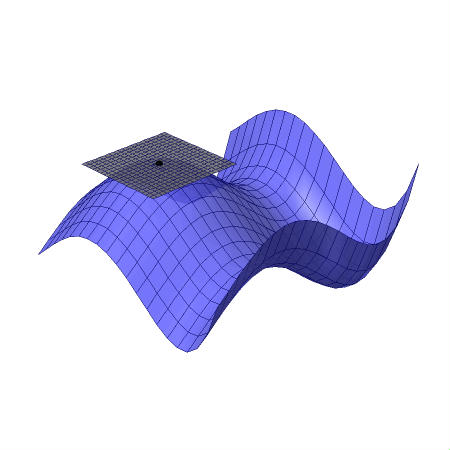
\includegraphics[width=200px]{loc-max.jpg}

\vspace{1cm}

\textsc{\LARGE University College London}\\[1.5cm]

\textsc{\Large Autumn Term 2014}\\[0.5cm]


% Title
\HRule \\[0.4cm]
{ \huge \bfseries Mathematical Methods 3}\\[0.4cm]

\HRule \\[1.5cm]

% Author
\begin{minipage}{0.4\textwidth}
\begin{flushleft} \large
Jonny Evans
\end{flushleft}
\end{minipage}
\begin{minipage}{0.4\textwidth}
\begin{flushright} \large

\includegraphics{by-sa.png}
\end{flushright}
\end{minipage}

\vfill

% Bottom of the page
{\large Last updated \today}

\end{center}

\end{titlepage}

%%%%%%%%%%%%%%%%%%%%%%%%%%%%%%%%%%%%%%%%%%%%%%%%%%%%%%%%%%%%%%%%%%%%%%%%%%%%%%%%%%%%%%%%%%%%%%%%%%%%%%%%%



\tableofcontents

\part{Fourier theory and separation of variables}

\chapter{Fourier series}


%%%%%%%
%
%\section{Notation}
%
%\[\delta_{mn}=\begin{cases}
%                      0   & \mbox{ if }n\neq m\\
%                      1   & \mbox{ if }n=m
%              \end{cases}\]
%%%%%%

\section{The heat equation}

\subsection{What is the heat equation}

The heat equation is a partial differential equation which governs the evolution of a temperature distribution on a one-dimensional rod. If the rod has length $L$ and is parametrised by a coordinate $x\in[0,L]$ and $t$ denotes time then the temperature at time $t$ at position $x$ on the rod is given by a function $\phi(x,t)$. The heat equation is
\[\pd{\phi}{t}=C\ppd{\phi}{x}\]
where $C$ is a constant (we will usually take $C=1$) depending on the material of which the rod is made (how well it conducts and heats up).

\subsection{Where does this equation come from?}

One can derive the heat equation from the following experimentally-observed facts: (a) Heat flows down a temperature gradient. Moreover, it flows at a rate proportional to the gradient $\pd{\phi}{x}$. Let us write $A$ for the constant of proportionality (conductivity). Thus the rate of change of heat energy is $-A\pd{\phi}{x}$ (the minus sign coming from the fact that heat flows {\em down} the gradient). (b) A quantity $\Delta H$ of heat energy will change the temperature of a segment of rod of length $\Delta x$ by $B\Delta H/\Delta x$ where $B$ is a constant (related to the ``specific heat capacity'' of the rod).

Given these two assumptions, if we focus on a small segment of rod between $x$ and $x+\Delta x$ for a short length of time $\Delta t$ then the amount of heat energy which flows in at the point $x$ is approximately $-A\pd{\phi}{x}(x)\Delta t$ and the amount which flows out at $x+\Delta x$ is $-A\pd{\phi}{x}(x+\Delta x)\Delta t$. Thus the total change in heat energy in this segment over the time interval $\Delta t$ is
\[\Delta H=A\Delta t\left(\pd{\phi}{x}(x+\Delta x)-\pd{\phi}{x}(x)\right).\]
This effects a change
\[\Delta\phi=AB\Delta t\frac{\left(\pd{\phi}{x}(x+\Delta x)-\pd{\phi}{x}(x)\right)}{\Delta x}\]
in temperature. Setting $C=AB$, dividing by $\Delta t$ and considering smaller and smaller time intervals and rod segments $\Delta x,\Delta t\to 0$, this expression limits to
\[\pd{\phi}{t}=C\ppd{\phi}{x}.\]

\subsection{How to solve it?}

Let's assume for simplicity that $C=1$ and fix boundary conditions $\phi(0,t)=\phi(\pi,t)=0$. We can spot a few solutions by inspection. For example
\[\phi_1(x,t)=\sin x e^{-t}\]
is a solution (check: $\pd{\phi}{t}=-\sin x e^{-t}$, $\ppd{\phi}{x}=-\sin x e^{-t}$ so $\phi$ satisfies the heat equation). So does
\[\phi_2(x,t)=\sin(2x)e^{-4t}\]
or, more generally,
\[\phi_n(x,t)=\sin(nx)e^{-n^2t}\]
(we'll see later how to get these solutions systematically instead of just guessing them).

Moreover the heat equation is linear: a linear combination of solution is again a solution. Indeed, under suitable convergence assumptions (allowing us to differentiate term-by-term) we can take an infinite linear combination
\[\phi(x,t)=\sum_{n=1}^{\infty}A_n\sin(nx)e^{-n^2t}\]
and the result is still a solution. So we have a vast bank of possible solutions, one for each (suitably convergent) infinite sequence $A_n$.

If we start off with an initial temperature distribution $\phi(x,0)=F(x)$ and fix the boundary conditions as above then we should know the temperature everywhere at all times, so which sequence $A_n$ do we need to pick to get the right solution? Let us substitute the solution into the initial condition:
\[F(x)=\phi(x,0)=\sum_{n=1}^{\infty}A_n\sin(nx)\]
(the $e^{-n^2t}$ terms are all equal to 1 at $t=0$). So the question becomes: given a function $F(x)$, when can we expand it as an infinite linear combination of sine functions? This was the question that Fourier found himself asking after precisely this line of reasoning.

\section{Fourier theory}

Fourier theory provides an expansion of a (more-or-less) arbitrary function $[-L,L]\to\RR$ in terms of sines and cosines.

\begin{thm}
Any sufficiently nice function $F\colon [-L,L]\to\RR$ can be written as a {\emph Fourier series}:
\[F(x)=c+\sum_{n=1}^{\infty}\left(a_n\fcos{n}+b_n\fsin{n}\right).\]
For example, any function on $[-\pi,\pi]$ can be written as
\[F(x)=c+\sum_{n=1}^{\infty}\left(a_n\cos(nx)+b_n\sin(nx)\right).\]
The $a_n,b_n,c$ are called the {\emph Fourier coefficients} of $F$.
\end{thm}

``Sufficiently nice'' could mean, for example, ``differentiable except at a finite collection of points''. When we say ``can be written as'' we mean that the series converges in some sense to the original function. We will not prove this theorem and will defer discussion of convergence till later. Instead, assuming that the theorem is true and that there are no convergence issues, let's work out what the Fourier coefficients would have to be. First we need a lemma.

\begin{lma}
If $n\geq 0$ is an integer then
\begin{align}
\label{eq:fsin}
\int_{-L}^L\fsin{n}dx        &= 0\\
\label{eq:fcos}
\int_{-L}^L\fcos{n}dx        &= 2L\delta_{n0}
\end{align}
If $m,n>0$ are integers then
\begin{align}
\label{eq:fsinfsin}
\int_{-L}^L\fsin{n}\fsin{m}dx&= L\delta_{mn}\\
\label{eq:fcosfcos}
\int_{-L}^L\fcos{n}\fcos{m}dx&= L\delta_{mn}\\
\label{eq:fcosfsin}
\int_{-L}^L\fcos{n}\fsin{m}dx&= 0.
\end{align}
\end{lma}
\begin{proof}[Proof of \eqref{eq:fsinfsin}]
Using the trigonometric identity
\[\cos(A-B)-\cos(A+B)=2\sin(A)\sin(B)\]
we can write the left-hand side of \eqref{eq:fsinfsin} as
\[
\frac{1}{2}\int_{-L}^L\fcos{(n-m)}dx-\frac{1}{2}\int_{-L}^L\fcos{(n+m)}dx
\]
Since we are assuming that $m,n>0$, we have $n+m\neq 0$ so, by \eqref{eq:fcos}, the second integral vanishes. Again, by \eqref{eq:fcos}, the first integral equals $\frac{1}{2}2L\delta_{mn}=L\delta_{mn}$.
\end{proof}

Using these formulae, we can find $c$, $a_n$ and $b_n$:

\begin{thm}\label{thm:fouco}
If
\[F(x)=c+\sum_{n=1}^{\infty}\left(a_n\fcos{n}+b_n\fsin{n}\right)\]
then
\begin{align}
\label{eq:fourierc}
   c   &    = \frac{1}{2L}\int_{-L}^LF(x)dx\\
\label{eq:fourierA}
   a_m &    = \frac{1}{L}\int_{-L}^LF(x)\fcos{m}dx\\
\label{eq:fourierB}
   b_m &    = \frac{1}{L}\int_{-L}^LF(x)\fsin{m}dx
\end{align}
\end{thm}
\begin{proof}[Proof of \eqref{eq:fourierc}]
\begin{align*}
 \int_{-L}^LF(x)dx
        & = \int_{-L}^{L}cdx
            + \sum_{n=1}^{\infty}\int_{-}^La_n\fcos{n}\\
&\qquad\qquad+ \sum_{n=1}^{\infty}\int_{-}^Lb_n\fsin{n}\\
        & = 2Lc
            + 0
            + 0
\end{align*}

so $c=\frac{1}{2L}\int_{-L}^LF(x)dx$.
\end{proof}
\begin{proof}[Proof of \eqref{eq:fourierA}]
\begin{align*}
 \int_{-L}^LF(x)\fcos{m}dx
        & = \int_{-L}^{L}c\fcos{m}dx
            + \sum_{n=1}^{\infty}\int_{-}^La_n\fcos{n}\fcos{m}\\
&\qquad\qquad+ \sum_{n=1}^{\infty}\int_{-}^Lb_n\fsin{n}\fcos{m}\\
        & = 0
            + L\sum_{n=1}^{\infty}\delta_{mn}a_n
            + 0\\
        & = La_m
\end{align*}

so

\[
  a_m = \frac{1}{L}\int_{-L}^LF(x)\fcos{m}dx
\]
\end{proof}

The proof of \eqref{eq:fourierB} is left as an exercise.

\begin{exm}\label{exm:fxequalsx}
Consider the function $F(x)=x$ on the interval $[-\pi,\pi]$ (i.e. $L=\pi$). Its Fourier coefficients are given by
\begin{align*}
c&=\frac{1}{2\pi}\int_{-\pi}^{\pi}xdx\\
&=\frac{1}{2\pi}\left[\frac{x^2}{2}\right]_{-\pi}^{\pi}\\
&=0\\
a_n&=\frac{1}{\pi}\int_{-\pi}^{\pi}x\cos nx dx\\
&=\frac{1}{\pi}\left(\left[x\frac{\sin(nx)}{n}\right]_{-\pi}^{\pi}-\int_{-\pi}^{\pi}\frac{\sin(nx)}{n}\right)\\
&=0+\frac{1}{n^2\pi}\left[\cos(nx)\right]_{-\pi}^{\pi}\\
&=0
\end{align*}
(where we have used $\sin(\pm\pi)=0$ and $\cos(n\pi)=\cos(-n\pi)$) and
\begin{align*}
b_n&=\frac{1}{\pi}\int_{-\pi}^{\pi}x\sin nx dx\\
&=\frac{1}{\pi}\left(\left[-x\frac{\cos(nx)}{n}\right]_{-\pi}^{\pi}+\int_{-\pi}^{\pi}\frac{\cos(nx)}{n}\right)\\
&=(-\cos(n\pi)/n-\cos(n\pi)/n)+\frac{1}{n^2\pi}\left[\sin(nx)\right]_{-\pi}^{\pi}\\
&=-2\cos(n\pi)/n\\
&=2(-1)^{n+1}/n
\end{align*}
where we have used that $\cos(n\pi)=(-1)^n$.

Therefore the Fourier series of $F(x)=x$ on $[-\pi,\pi]$ is
\[x=2\sum_{n=1}^{\infty}\frac{(-1)^{n+1}}{n}\sin(nx),\]
that is
\[x=2\left(\frac{\sin(x)}{1}-\frac{\sin(2x)}{2}+\frac{\sin(3x)}{3}-\cdots\right)\]
We should think of this as an infinite series of approximations to $x$, obtained by truncating the sum after finitely many terms. We plot the graphs of these truncations in Figure \ref{fig:fourier-x} below and you can see that the graphs are tending (in some fairly weak sense) to the graph of the straight line.
\end{exm}

\begin{figure}
\label{fig:fourier-x}
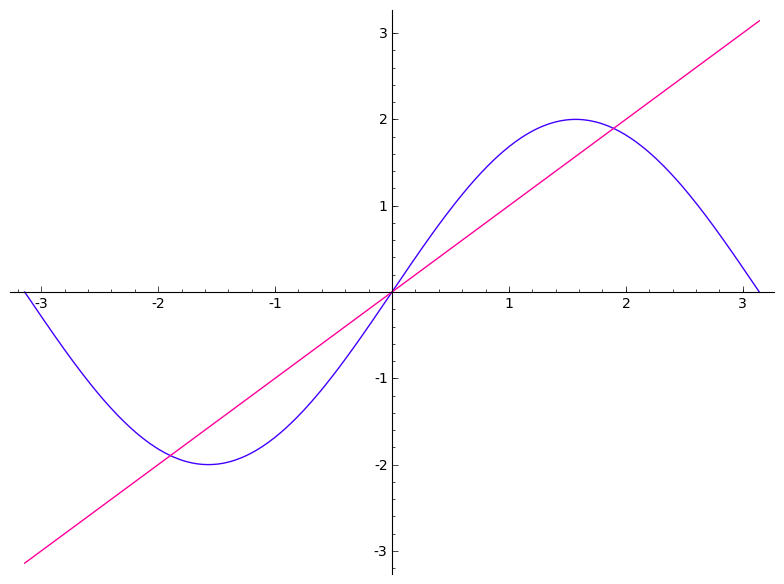
\includegraphics[width=200px]{fourier-1.png}
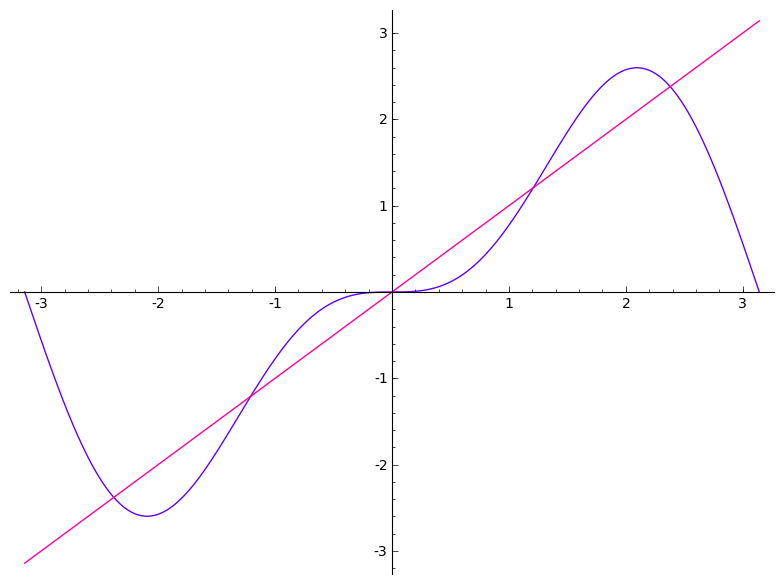
\includegraphics[width=200px]{fourier-2.png}
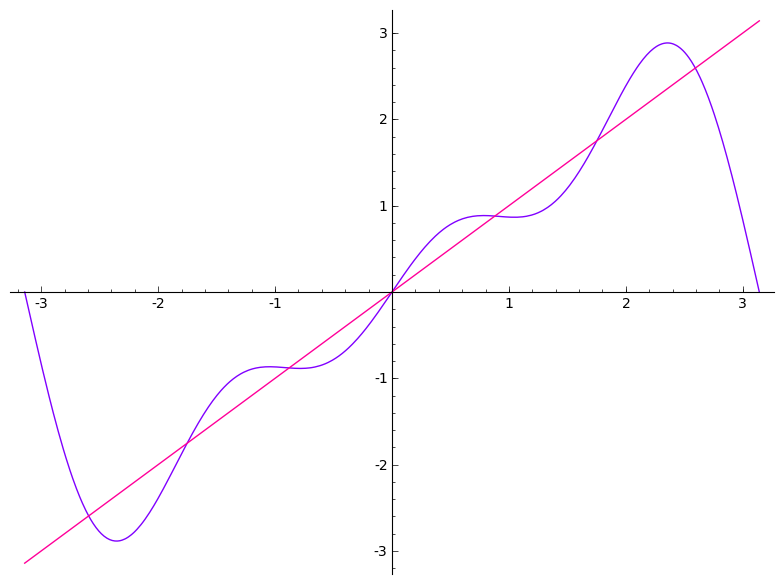
\includegraphics[width=200px]{fourier-3.png}
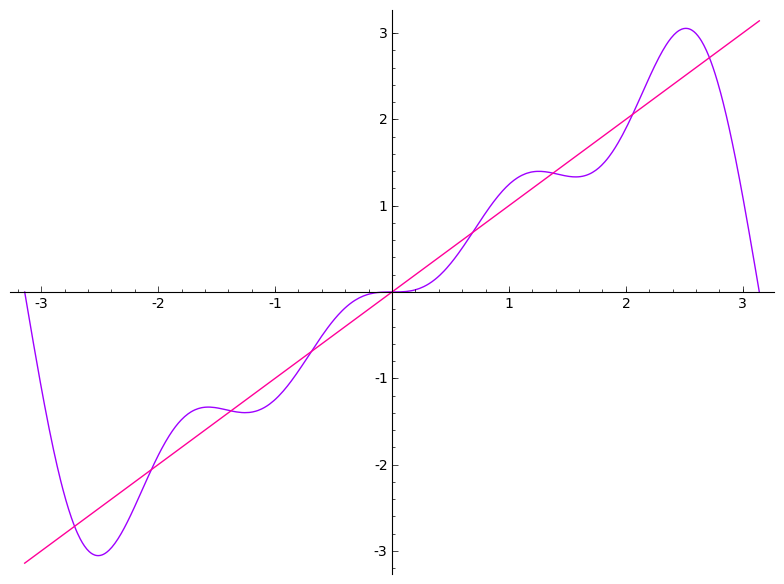
\includegraphics[width=200px]{fourier-4.png}
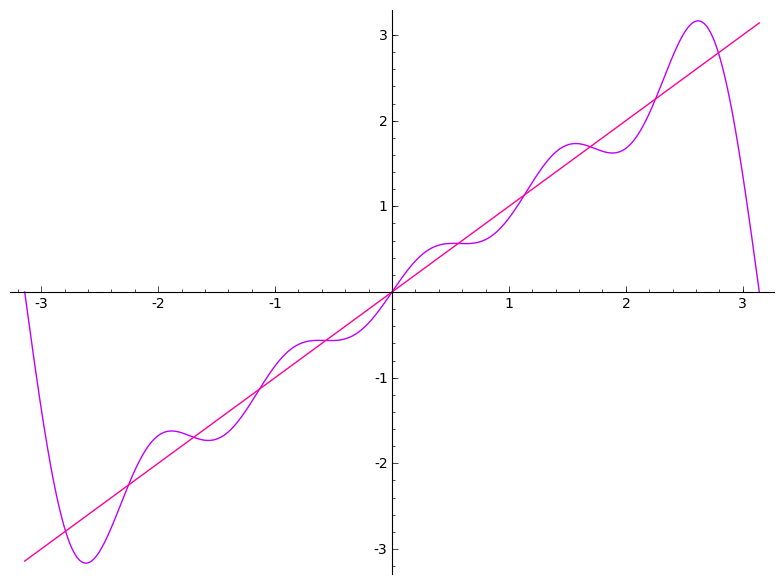
\includegraphics[width=200px]{fourier-5.png}
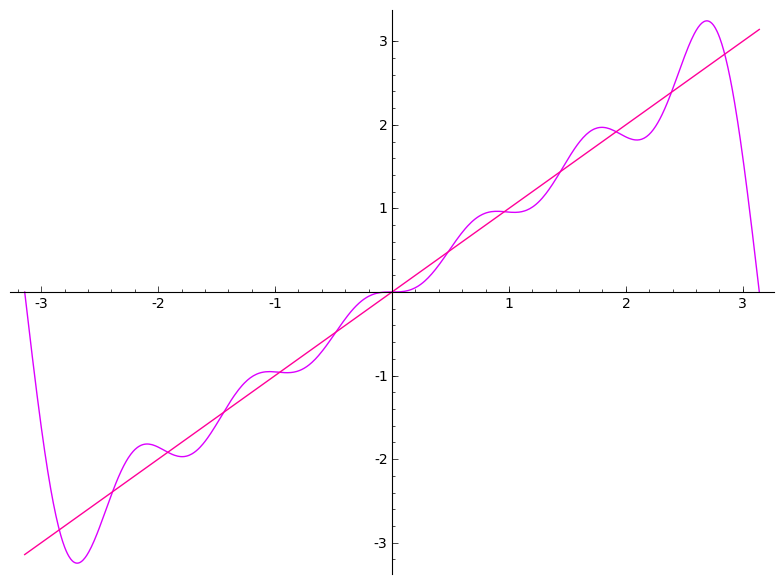
\includegraphics[width=200px]{fourier-6.png}
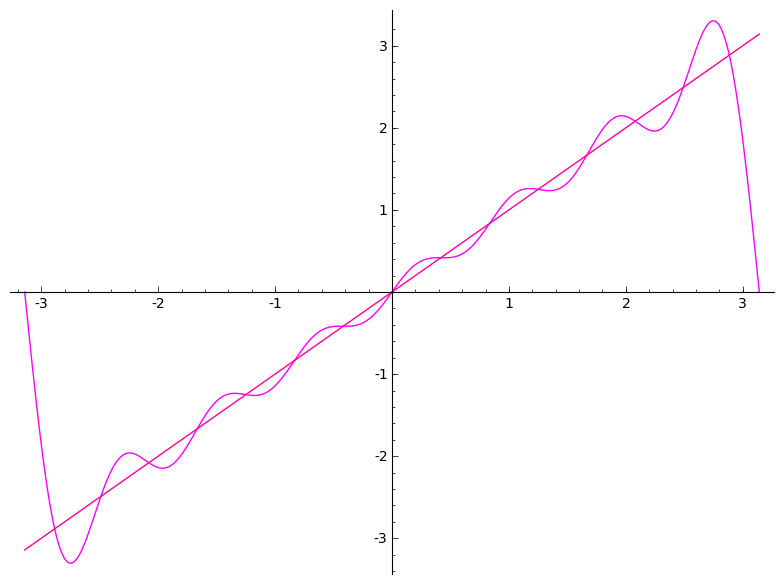
\includegraphics[width=200px]{fourier-7.png}
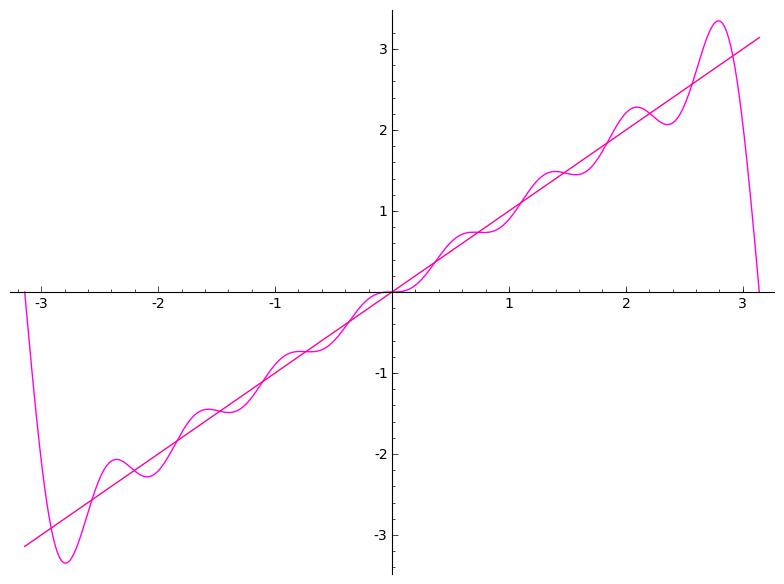
\includegraphics[width=200px]{fourier-8.png}
\caption{The graphs of $2\sum_{n=1}^N\frac{(-1)^{n+1}}{n}\sin(nx)$ for $N=1,2,3,4,5,6,7,8$.}
\end{figure}

Notice that there is a shortcut to computing Fourier series when the function has certain symmetries. A function $F$ is {\em odd} if $F(-x)=-F(x)$ and {\em even} if $F(-x)=F(x)$ (so $F(x)=x$ is odd and $F(x)=\cos(x)$ is even).
\begin{lma}
Suppose $F$ has Fourier series.
\[F(x)=c+\sum_{n=1}^{\infty}\left(a_n\fcos{n}+b_n\fsin{n}\right)\]
If $F$ is even then:
\begin{itemize}
\item $b_n=0$,
\item $a_n=\frac{2}{L}\int_0^LF(x)\fcos{n}dx$,
\item $c=\frac{1}{L}\int_0^LF(x)dx$.
\end{itemize}
If $F$ is odd then:
\begin{itemize}
\item $b_n=\frac{2}{L}\int_0^LF(x)\fsin{n}dx$,
\item $a_n=0$,
\item $c=0$.
\end{itemize}
\end{lma}
We saw this in the previous example: $F(x)=x$ is odd and we found $a_n=c=0$.
\begin{proof}[Proof of Lemma]
Let us show that $F(x)$ even implies $b_n=0$ (the other proofs proceed in exactly the same way).

We have
\begin{align*}
b_n&=\frac{1}{L}\int_{-L}^LF(x)\fsin{n}dx\\
   &=\frac{1}{L}\left(\int_{-L}^0F(x)\fsin{n}dx+\int_0^LF(x)\fsin{n}dx\right)
\end{align*}
(that is we split the range of the integral in half and perform each half separately). Substituting $u=-x$ in the first integral gives
\[\int_{-L}^0F(x)\fsin{n}dx=\int_{L}^0F(-u)\sin\left(\frac{-n\pi u}{L}\right)(-du)\]
using $F(-u)=F(u)$ (evenness) and $\sin(-n\pi u/L)=-\sin(n\pi u/L)$ we get
\[\int_L^0F(u)\sin\left(\frac{n\pi u}{L}\right)du\]
or
\[-\int_0^LF(u)\sin\left(\frac{n\pi u}{L}\right)du\]
(swapping the limits of the integral swaps the sign). Therefore
\[b_n=-\int_0^LF(u)\sin\left(\frac{n\pi u}{L}\right)du+\int_0^LF(x)\sin\left(\frac{n\pi x}{L}\right)dx=0\]
as required.
\end{proof}

\begin{exm}
Consider ($L=1$)
\[F(x)=\begin{cases}0&\mbox{ if }x\in[-1,0)\\ \tfrac{1}{2}&\mbox{ if }x=0\\1&\mbox{ if }x\in(0,1].\end{cases}\]
This function is neither odd nor even, but if we subtract $1/2$ then we get an odd function
\[G(x)=\begin{cases}-\tfrac{1}{2}&\mbox{ if }x\in[-1,0)\\ 0&\mbox{ if }x=0\\\tfrac{1}{2}&\mbox{ if }x\in(0,1].\end{cases}\]
This has Fourier coefficients
\begin{align*}
b_n&=2\int_0^1G(x)\sin(n\pi x)dx\\
   &=\int_0^1\sin(n\pi x)dx\\
   &=\frac{1}{n\pi}[-\cos(n\pi x)]_0^1\\
   &=\frac{1-(-1)^n}{n\pi}.
\end{align*}
That means that $b_n=2/n\pi$ if $n$ is odd and zero if $n$ is even. Therefore $G(x)=\frac{2}{\pi}\sin(\pi x)+\frac{2}{3\pi}\sin(3\pi x)+\cdots$ and
\[F(x)=\frac{1}{2}+\frac{2}{\pi}\sin(\pi x)+\frac{2}{3\pi}\sin(3\pi x)+\cdots\]
\end{exm}

\begin{exm}\label{exm:fxequalsxsquared}
Consider $F(x)=x^2$ on the interval $[-\pi,\pi]$. This function is even so $b_n=0$ automatically. We have
\[c=\frac{1}{\pi}\int_0^{\pi}x^2dx=\frac{\pi^3}{3}\]
and
\begin{align*}
a_n&=\frac{2}{\pi}\int_0^{\pi}x^2\cos(nx)dx\\
   &=\frac{2}{\pi}\left(\cancelto{0}{\left[x^2\frac{\sin(nx)}{n}\right]_0^{\pi}}-\frac{2}{n}\int_0^{\pi}x\sin(nx)dx\right)\\
   &=-\frac{4}{n\pi}\left(\left[-x\frac{\cos(nx)}{n}\right]_0^{\pi}+\frac{1}{n}\int_0^{\pi}\cos(nx)dx\right)\\
   &=\frac{4}{n^2}(-1)^n-\cancelto{0}{\frac{1}{n}\left[-\frac{\sin(nx)}{n}\right]_0^{\pi}}\\
   &=\frac{4(-1)^n}{n^2}
\end{align*}
therefore
\[x^2=\frac{\pi^2}{3}-4\left(\cos x-\frac{\cos 2x}{4}+\frac{\cos 3x}{9}-\cdots\right)\]
on $[-\pi,\pi]$.
\end{exm}

\subsection{Half-range Fourier series}

Often we only specify the values of a function on the interval $[0,L]$ and we only want to see sine terms in its Fourier expansion (we will see this when we solve the heat equation).

\begin{dfn}
Suppose that $F(x)$ is a function $[0,L]\to\RR$. Define its {\em odd extension} to be the function
\[F_{even}(x)=\begin{cases}F(x)&\mbox{ if }x>0\\ -F(-x)&\mbox{ if }x<0.\end{cases}\]
The half-range sine series of $F$ is then defined to be the Fourier series of $F_{even}$, in other words
\[F(x)=\sum_{n=1}^{\infty}b_n\fsin{n}\]
on $[0,L]$ where $b_n=\frac{2}{L}\int_0^LF(x)\fsin{n}dx$.
\end{dfn}
Analogously one can define the half-range cosine series by taking the Fourier series of the even extension
\[F_{odd}(x)=\begin{cases}F(x)&\mbox{ if }x>0\\ F(-x)&\mbox{ if }x<0.\end{cases}\]

\begin{exm}\label{exm:xpiminusxsquared}
Consider the function $F(x)=x(\pi-x)$ on the interval $[0,\pi]$. We have
\begin{align*}
b_n&=\frac{2}{\pi}\int_0^{\pi}x(\pi-x)\sin(nx)dx\\
   &=\frac{2}{\pi}\left(\cancelto{0}{\left[-x(\pi-x)\frac{\cos(nx)}{n}\right]_0^{\pi}}+\frac{1}{n}\int_0^{\pi}(\pi-2x)\cos(nx)dx\right)\\
   &=\frac{2}{n\pi}\left(\left[(\pi-2x)\frac{\sin(nx)}{n}\right]_0^{\pi}+\frac{1}{n}\int_0^{\pi}2\sin(nx)dx\right)\\
   &\frac{4((-1)^{n+1}+1)}{n^3\pi}\\
   &=\begin{cases}
       \frac{8}{n^3\pi}&\mbox{ if }n\mbox{ is odd}\\
       0&\mbox{ if }n\mbox{ is even}
     \end{cases}
\end{align*}
so
\[x(\pi-x)=8\left(\frac{\sin x}{\pi}\sin x+\frac{\sin 2x}{8\pi}+\frac{\sin 3x}{27\pi}+\cdots\right)\]
on $[0,\pi]$. Note that in this example, although the function $x(\pi-x)$ is not odd (or even!), we are taking its odd extension and computing the Fourier series of that which is why only sine terms appear. This is what we call the half-range sine series.
\end{exm}

\section{Parseval's theorem}

\begin{thm}[Parseval's theorem]
If $F(x)=c+\sum_{n=1}^{\infty}\left(a_n\fcos{n}+b_n\fsin{n}\right)$ then
\[\frac{1}{L}\int_{-L}^LF(x)^2dx=2c^2+\sum_{n=1}^{\infty}(a^2_n+b^2_n).\]
\end{thm}
\begin{proof}
We have:
\begin{align*}
\frac{1}{L}\int_{-L}^LF(x)^2dx&=\frac{1}{L}\int_{-L}^LF(x)\left(c+\sum_{n=1}^{\infty}\left(a_n\fcos{n}+b_n\fsin{n}\right)\right)dx\\
     &=\frac{c}{L}\int_{-L}^LF(x)dx+\sum_{n=1}^{\infty}\frac{a_n}{L}\int_{-L}^LF(x)\fcos{n}dx+\sum_{n=1}^{\infty}\frac{b_n}{L}\int_{-L}^LF(x)\fsin{n}dx\\
&=2c^2+\sum_{n=1}^{\infty}(a^2_n+b^2_n)
\end{align*}
using the formulae for $c,a_n,b_n$ given in Theorem \ref{thm:fouco}.
\end{proof}

\begin{cor}
We have
\[\frac{\pi^2}{6}=\sum_{n=1}^{\infty}\frac{1}{n^2}.\]
\end{cor}
\begin{proof}
Take $F(x)=x$ on $[-\pi,\pi]$. We computed the Fourier series of $F(x)$ on $[-\pi,\pi]$ in Example \ref{exm:fxequalsx} and found
\[F(x)=\sum_{n=1}^{\infty}\frac{2(-1)^{n+1}}{n}\sin(nx).\]
Applying Parseval's theorem implies that
\[\frac{1}{\pi}\int_{-\pi}^{\pi}x^2dx=\sum_{n=1}^{\infty}\frac{4}{n^2}\]
and the left-hand side equals $2\pi^2/3$. Rearranging gives the desired relationship.
\end{proof}

\begin{cor}
We have
\[\frac{\pi^4}{90}=\sum_{n=1}^{\infty}\frac{1}{n^4}.\]
\end{cor}
\begin{proof}
Take $F(x)=x^2$ on $[-\pi,\pi]$. We computed the Fourier series of $F(x)$ on $[-\pi,\pi]$ in Example \ref{exm:fxequalsxsquared} and found
\[F(x)=\frac{\pi^2}{3}+\sum_{n=1}^{\infty}\frac{4(-1)^n}{n^2}\cos(nx).\]
Applying Parseval's theorem implies that
\[\frac{1}{\pi}\int_{-\pi}^{\pi}x^4dx=\frac{2\pi^4}{9}+\sum_{n=1}^{\infty}\frac{16}{n^4}\]
The left-hand side equals $\frac{2\pi^4}{5}$ so rearranging gives
\[\frac{\pi^4}{90}=\frac{1}{16}\left(\frac{2\pi^4}{5}-\frac{2\pi^4}{9}\right)=\sum_{n=1}^{\infty}\frac{1}{n^4}\]
as required.
\end{proof}

In general, when it converges, the sum $\zeta(s):=\sum_{n=1}^{\infty}\frac{1}{n^s}$ is called the {\em Riemann zeta function} so we have evaluated $\zeta(2)=\frac{\pi^2}{6}$ and $\zeta(4)=\frac{\pi^4}{90}$.

\section{The Hilbert space picture}

\subsection{An analogy}

Parseval's theorem says that
\[F(x)=c+\sum_{n=1}^{\infty}\left(a_n\fcos{n}+b_n\fsin{n}\right)\]
implies
\[\frac{1}{L}\int_{-L}^LF(x)^2dx=2c^2+\sum_{n=1}^{\infty}(a^2_n+b^2_n).\]
This looks a little bit like Pythagoras's theorem, which says that
\[v=ae_1+be_2\]
implies that
\[|v|^2=a^2+b^2.\]
Here $e_1$ and $e_2$ are an orthonormal basis for $\RR^2$ and $|v|^2$ denotes the squared length of the vector $v$.

To make this analogy precise, we should consider $F$ as a vector in a vector space. Which vector space? The vector space of real-valued functions on $[-L,L]$! You can add functions, you can multiply them by real numbers and they obey the axioms (e.g. distributivity) required to form a vector space.

Then we should think of $1$ (the constant function), $\fcos{n}$ and $\fsin{n}$ as basis vectors in this space of functions. When we write $F$ as a Fourier series we are expanding in terms of this basis. Notice that in the definition of ``basis'' we are only allowed to take finite linear combinations of basis vectors, so Fourier series are something more general. We say that $1,\fcos{n},\fsin{n}$ form a {\em Hilbert space basis} for the space of functions.

Notice that since our basis consists of infinitely many (linearly independent) functions, our vector space must be infinite-dimensional.

We should also think of $\frac{1}{L}\int_{-L}^LF(x)^2dx$ as the ``length'' of the vector $F$. Indeed we will think of
\[\left\langle F,G\right\rangle:=\frac{1}{L}\int_{-L}^LF(x)G(x)dx\]
as a ``dot product'' (or {\em inner product}) between functions $F$ and $G$ thought of as vectors in the vector space of functions. With respect to this inner product, the basis vectors $1$, $\fcos{n}$ and $\fsin{n}$ satisfy orthogonality relations
\begin{align*}
\left\langle \fsin{n},\fcos{m}\right\rangle&=\frac{1}{L}\int_{-L}^L\fsin{n}\fcos{m}dx=0\\
\left\langle \fsin{n},1\right\rangle&=\frac{1}{L}\int_{-L}^L\fsin{n}=0\\
\left\langle \fcos{n},1\right\rangle&=\frac{1}{L}\int_{-L}^L\fcos{n}=0\\
\left\langle \fsin{n},\fsin{m}\right\rangle&=\frac{1}{L}\int_{-L}^L\fsin{n}\fsin{m}dx=\delta_{mn}\\
\left\langle \cos{n},\fcos{m}\right\rangle&=\frac{1}{L}\int_{-L}^L\fcos{n}\fcos{m}dx=\delta_{mn}\\
\left\langle 1,1\right\rangle&=\frac{1}{L}\int_{-L}^Ldx=2
\end{align*}
by the Fourier integral identities! This makes it {\em almost} an orthonormal basis - the only problem being that $1$ has length $2$. Normalising this we get a unit vector $1/\sqrt{2}$. This accounts for the random factor of 2 that crops up in Parseval's theorem in front of $c^2$.

In general a (real\footnote{There are also complex Hilbert spaces.}) {\em Hilbert space} is a vector space over $\RR$ with an inner product satisfying:
\begin{itemize}
\item $\langle x,y\rangle=\langle y,x\rangle$,
\item $\langle ax+by,z\rangle=a\langle x,z\rangle+b\langle y,z\rangle$,
\item $\|x\|^2:=\langle x,x\rangle\geq 0$ with equality if and only if $x=0$,
\item the space is {\em complete} in the following sense. Suppose that $v_k$ is a sequence of vectors such that $\sum_{k=1}^N\|v_k\|^2<\infty$. Then there exists a vector $v$ such that
\[\left\|v-\sum_{k=1}^{N}v_k\right\|\to 0\]
as $N\to\infty$.
\end{itemize}
This final axiom is the important one. It allows us to make sense of infinite sums like Fourier series.

\subsection{A word about convergence}

Note that $\left\langle F,F\right\rangle$ only makes sense if $F^2$ is integrable. So we should restrict to functions for which $\int_{-L}^LF(x)^2dx$ exists and is finite. These are called $L^2$-functions and the inner product $\left\langle,\right\rangle$ is called the $L^2$-inner product ($\left\langle F,F\right\rangle$ is called the $L^2$-norm of $F$). We often write $\|F\|^2=\left\langle F,F\right\rangle$.

The convergence of a Fourier series to $F$ is to be understood in the $L^2$ sense, that is if $F_N=c+\sum_{n=1}^N\left(a_n\fcos{n}+b_n\fsin{n}\right)$ then
\[\|F-F_N\|^2\to 0\mbox{ as }N\to\infty.\]
This is a relatively weak notion of convergence. It means that the squared difference between the function and its $N$th Fourier approximation is small {\em on average} (but not necessarily small everywhere). This is known as a least-squares approximation. There are certainly examples where, for some $x$, $F_N(x_0)$ does not converge to $F(x_0)$ as $N\to\infty$. This happens for example at a discontinuity of $F$ (see the pictures of the Fourier series of $F(x)=x$ on $[-\pi,\pi]$, for example - you can think of this as having a discontinuity at $\pm\pi$ because if you wrap back around then the function jumps down from $\pi$ to $-\pi$). The least-squares convergence means that the region in which the function is poorly-approximated gets smaller and smaller as $N$ increases.

For some functions (e.g. differentiable functions) the Fourier series does converge pointwise everywhere (i.e. $F_N(x_0)\to F(x_0)$ for all $x_0$). Here differentiability is understood to mean that even if we extend $F$ periodically to the whole of $\RR$ by setting $F(x+2nL)=F(x)$, then the result is differentiable (this is not the case for $F(x)=x$).



\iffalse
\section{Examples}

\begin{exm}[The saw-tooth wave]
The function $G(x)=x$ is not $2L$-periodic. However, there is a $2L$-periodic function $F(x)=x-2L[x/2L]-L$ which agrees with $G(x)$ on $[-L,L]$. It is easier t imagine its graph: take the graph of $G(x)=x$ on $[-L,L]$ and translate it to live over $\ldots,[-5L,-3L],[-3L,-L],[-L,L],[L,3L],[3L,5L],\ldots$ to get a ``saw-tooth wave''. We will now compute the Fourier coefficients of $F(x)$.

\begin{align*}
  c  & = \int_{-L}^Lxdx\\
     & = \left[\frac{x^2}{2}\right]_{-L}^L\\
     & = 0
\end{align*}

\begin{align*}
  A_n &=
\end{align*}
\end{exm}



In fact, {\emph any} function $G$ whose domain of definition includes the interval $[-L,L]$ can be used to generate a $2L$-periodic function $F(x)=G(x-2L[x/2L]-L)$ which agrees with $G$ on the interval $[-L,L]$. The moral of this is: whenever I take the Fourier expansion of a function $G$ which seems not to be periodic (like $G(x)=x$ or $G(x)=x^2$) I am really taking the Fourier expansion of the unique periodic function which agrees with $G$ on $[-L,L]$.

\begin{exm}[The square wave]
The function $G(x)=\begin{cases}0&\mbox{ if }x<0\\ 1&\mbox{ if }x\geq 1\end{cases}$ gives a $2L$-periodic function $F(x)=G(x-2L[x/2L]-L)$ whose graph looks like a ``square wave''.
\end{exm}

\fi

\chapter{Separation of variables}

\section{Separation of variables for the heat equation}

When we explained how to solve the heat equation we guessed an infinite collection of solutions $\sin nx e^{-n^2t}$. In this section we will see how to derive these solutions systematically.

\subsection{Separating variables}

\begin{dfn}
A {\em separated solution} to the heat equation is a solution which has the form $\phi(x,t)=X(x)T(t)$ (where $X$ is a function depending only on $x$ and $T$ is a function depending only on $t$). We will denote the derivative $dX/dx$ by $X'$ and the derivative $dT/dt$ also by $T'$; in other words, a prime on a function of a single variable means ``differentiate with respect to the variable''.
\end{dfn}

\begin{lma}\label{lma:sepvar}
If $XT$ is a separated solution then there is a constant $\lambda$ such that $X''=-\lambda X$ and $T'=-\lambda T$ (the minus sign is just a convention to make our lives easier later).
\end{lma}
\begin{proof}
The heat equation states that
\[\pd{\phi}{t}=\ppd{\phi}{x}.\]
Differentiating $XT$ with respect to $t$ gives $XT'$. Differentiating twice with respect to $x$ give $X''T$. Therefore the heat equation implies
\[XT'=X''T.\]
Dividing through by $XT$ gives
\[\frac{T'}{T}=\frac{X''}{X}.\]
We define this quantity to be $-\lambda(x,t)$. Since $-\lambda(x,t)=X''/X$ does not depend on $t$ and $-\lambda(x,t)=T'/T$ does not depend on $x$, we see that $\lambda$ is constant.
\end{proof}

\subsection{Solving for the separated solutions}

Solving the two ordinary differential equations in Lemma \ref{lma:sepvar} we get:

\begin{cor}
If $XT$ is a separated solution to the heat equation then $T=e^{-\lambda t}$ and
\[
X=\begin{cases}
  A\cos px+B\sin px&\mbox{ if }\lambda=p^2>0\\
  Ax+B&\mbox{ if }\lambda=0\\
  A\cosh px+B\sinh px&\mbox{ if }\lambda=-p^2<0.
\end{cases}
\]
\end{cor}

\subsection{Fitting to boundary conditions}

We now have a large array of separated solutions. To narrow this down we will impose some boundary conditions at the ends of the rod. Two common boundary conditions are:
\begin{itemize}
\item Dirichlet boundary conditions (where you specify the values of $\phi$ at the endpoints of the rod):
\[\phi(0,t)=M,\quad\phi(L,t)=N.\]
This means that we keep the endpoints of the rod at constant temperature.
\item Neumann boundary conditions (where you specify the values of the derivative $\pd{\phi}{x}$ at the endpoints of the rod):
\[\pd{\phi}{x}(0,t)=0,\quad\pd{\phi}{x}(L,t)=0.\]
Since the flow of heat is proportional to the gradient of $\phi$ this implies that there is no heat flowing out of the ends of the rod, i.e. the ends are insulated.
\end{itemize}
To find a unique solution to the heat equation we will also need to impose an initial condition $\phi(x,0)=F(x)$ for some function $F$.

\begin{rmk}\label{rmk:modify}
We can make a modification to assume $M=N=0$. If $\phi(x,t)$ is a solution to the heat equation satisfying the Dirichlet conditions
\[\phi(0,t)=M,\quad\phi(L,t)=N,\quad\phi(x,0)=F(x)\]
and $\phi_0(x,t)=M+\frac{N-M}{L}x$ then $\theta(x,t)=\phi(x,t)-\phi_0(x,t)$ is a solution of the heat equation satisfying the boundary conditions
\[\theta(0,t)=\theta(L,t)=0,\quad\theta(x,0)=F(x)-\phi_0(x,0).\]
Note that $\theta$ is a linear combination of solutions to the heat equation, so it is automatically a solution since the equation is linear.
\end{rmk}

For a separated solution $\phi=XT$ to satisfy the Dirichlet conditions $\phi(0,t)=\phi(L,t)=0$ implies $X(0)T(t)=X(L)T(t)=0$ for all $t$, so $X(0)=X(L)=0$ or $T\equiv 0$. We are not interested in the trivial solution $\phi=0$, so let us examine the consequences of imposing $X(0)=X(L)=0$.

\begin{lma}\label{lma:dirichlet}
A separated solution $XT$ of the heat equation satisfying $X(0)=X(L)=0$ has the form
\[B\fsin{n}e^{-n^2\pi^2t/L^2}.\]
\end{lma}
\begin{proof}
If $\lambda=-p^2<0$ then the boundary conditions imply:
\begin{align*}
0&=A\cosh(0)+B\sinh(0)\\
 &=A\ \Rightarrow A=0,\\
0&=A\cosh(pL)+B\sinh(pL)\\
 &=B\sinh(pL)\mbox{ as }A=0\\
 &\Rightarrow B=0\mbox{ as }\sinh(pL)\neq 0.
\end{align*}
so the only possibility is the trivial solution $A=B=0$.

If $\lambda=0$ then the boundary conditions imply:
\begin{align*}
0&=A\times 0+B\\
 &=B\ \Rightarrow B=0,\\
0&=AL+B\\
 &=AL\mbox{ as }B=0\\
 &\Rightarrow A=0.
\end{align*}

Finally, if $\lambda=p^2>0$ then the boundary conditions imply:
\begin{align*}
0&=A\cos 0+B\sin 0\\
 &=A\ \Rightarrow A=0,\\
0&=A\cos pL+B\sin pL\\
 &=B\sin pL\mbox{ as }A=0\\
 &\Rightarrow B=0\mbox{ or }\sin pL=0.
\end{align*}
The only way to get a nontrivial solution is therefore if $\sin pL=0$ or $pL=n\pi$ for some $n\in\ZZ$. Therefore $X=B\fsin{n}$ and $T=e^{-n^2\pi^2t/L^2}$.
\end{proof}

Neumann conditions translate into $X'(0)=X'(L)=0$.

\begin{lma}
A separated solution $XT$ of the heat equation satisfying $X'(0)=X'(L)=0$ has the form
\[A\fcos{n}e^{-n^2\pi^2t/L^2}.\]
\end{lma}
\begin{proof}
Exercise.
\end{proof}

\subsection{Ansatz}

We can now take an arbitrary linear combination of separated solutions and the result is again a solution to the heat equation by linearity of the heat equation. Our strategy in solving the heat equation will therefore be: guess that the final solution has the form
\[\phi(x,t)=\sum_{n=1}^{\infty}B_n\fsin{n}e^{-n^2\pi^2t/L^2}\]
and try to choose the coefficients $B_n$ to fit the initial condition $\phi(x,0)=F(x)$. This is called making an {\em Ansatz} (``an educated guess that is later verified by its results'' - Wikipedia).

\subsection{Fitting to initial conditions}

Substituting the Ansatz into the initial condition gives
\[F(x)=\phi(x,0)=\sum_{n=1}^{\infty}B_n\fsin{n}\]
because $e^{-n^2\pi^20/L^2}=1$. Therefore we see that $B_n$ is the $n$th coefficient in the half-range Fourier sine series for $F(x)$.

\subsection{Examples}

\begin{exm}
{\bf Solve the heat equation with the initial condition $\phi(x,0)=-x^2$ and the Dirichlet boundary conditions $\phi(0,t)=0$, $\phi(\pi,t)=-\pi^2$.}

We have $M=0$, $N=-\pi^2$ so $\phi_0(x,t)=-\pi x$. Therefore $\phi=\phi_0+\theta$ where $\theta$ solves the heat equation with the initial condition $\theta(x,0)=-x^2-(-\pi x)=x(\pi-x)$ and the boundary conditions $\theta(0,t)=\theta(\pi,t)=0$. We make the Ansatz $\theta(x,t)=\sum_{n=1}^{\infty}B_n\sin(nx)e^{-n^2t}$ for $\theta$ and substitute in the initial condition $\theta(x,0)=x(\pi-x)$ to get
\[x(\pi-x)=\sum_{n=1}^{\infty}B_n\sin(nx).\]
Therefore $B_n$ is the $n$th Fourier coefficient of $x(\pi-x)$, which we found in Example \ref{exm:xpiminusxsquared} to be
\[B_n=\frac{4}{n^3\pi}((-1)^{n+1}+1).\]
Therefore the final solution is
\[\phi(x,t)=-\pi x+\sum_{n=1}^{\infty}\frac{4}{n^3\pi}((-1)^{n+1}+1)\sin(nx)e^{-n^2t}.\]
\end{exm}

\begin{rmk}
Notice that the higher Fourier modes (the terms with large $n$ in the sum) decay like $e^{-n^2t}$, faster than when $n$ is small. Physically this makes sense: heat flows down a temperature gradient and when $n$ is large, $\sin(nx)$ is very wiggly (it has large gradient). Therefore heat flows more quickly to even out the temperature distribution. As $t\to\infty$ the distribution tends to the linear temperature distribution $-\pi x$ (a so-called {\em steady} solution to the heat equation because it does not depend on $t$).
\end{rmk}
\begin{rmk}
If $\lambda<0$ then $e^{-\lambda t}$ would quickly get large. This would be unphysical: temperature distributions don't just spontaneously get hotter! This shows that the choice of boundary conditions is an important part of the physical input into the problem.
\end{rmk}

\begin{exm}
{\bf Solve the heat equation with the Neumann conditions $\pd{\phi}{x}(0,t)=\pd{\phi}{x}(\pi,t)=0$ and the initial condition $\phi(x,0)=\sin^2x$.}

In this example we don't need to modify with a $\phi_0$ term but we do need to use $A\cos(nx)e^{-n^2t}$ rather than the sine solution like the previous example, because we are using Neumann conditions. Note that by trigonometry we have $\sin^2x=\frac{1}{2}(1-\cos(2x))$ which is the half-range Fourier cosine series of $\sin^2x$ (there's only one way to express a given function as a Fourier cosine series and this is it for $\sin^2x$).

The Ansatz is
\[\phi(x,t)=\sum_{n=1}^{\infty}A_n\cos(nx)e^{-n^2t}\]
and the initial condition gives
\[\sin^2x=\phi(x,0)=\sum_{n=1}^{\infty}A_n\cos(nx)\]
so, comparing with the Fourier series $\sin^2x=\frac{1}{2}(1-\cos(2x))$ we see that $A_0=\frac{1}{2}$, $A_2=-\frac{1}{2}$ and all other coefficients vanish. Therefore
\[\phi(x,t)=\frac{1}{2}-\frac{1}{2}\cos(2x)e^{-4t}.\]
\end{exm}

\section{Separation of variables: the general strategy}

\begin{itemize}
\item Separate variables and find the separated solutions.
\item Determine which separated solutions satisfy the boundary conditions.
\item Form an Ansatz for the general solution by taking an infinite linear combination of the separated solutions satisfying the boundary conditions.
\item Choose the coefficients in the Ansatz to fit the initial conditions.
\end{itemize}

Sometimes one also needs to modify the problem by subtracting off a simple (e.g. linear) solution to make the boundary conditions amenable to solution by the Ansatz. For example, we saw this in Remark \ref{rmk:modify} and we will see it again! 

\section{The wave equation}

The wave equation is
\[\frac{1}{c^2}\ppd{\phi}{t}=\ppd{\phi}{x}\]
where $c$ is a constant called the wave speed. It describes
\begin{itemize}
\item vibrations in a one-dimensional string,
\item waves in water,
\item electromagnetic waves.
\end{itemize}
In each case, $\phi(x,t)$ describes the displacement (vertical displacement of the string or of the water surface, displacement of the electric or magnetic field away from zero) at the point $x$ at time $t$. We will derive it later from a variational principle: the string is trying to find the optimal balance between its kinetic energy and internal tension potential energy.

If $\phi(x,t)=X(x)T(t)$ is a separated solution then
\[\frac{1}{c^2}XT''=X''T\]
so $\frac{T''}{c^2T}=\frac{X''}{X}=-\lambda$ is a constant. Therefore $X''=-\lambda X$, giving
\[
X=\begin{cases}
  A\cos px+B\sin px&\mbox{ if }\lambda=p^2>0\\
  Ax+B&\mbox{ if }\lambda=0\\
  A\cosh px+B\sinh px&\mbox{ if }\lambda=-p^2<0,
\end{cases}
\]
and $T''=-c^2\lambda T$, giving
\[
T=\begin{cases}
  C\cos pct+D\sin pct&\mbox{ if }\lambda=p^2>0\\
  Ct+D&\mbox{ if }\lambda=0\\
  C\cosh pct+D\sinh pct&\mbox{ if }\lambda=-p^2<0.
\end{cases}
\]
The boundary conditions we will impose are either Dirichlet conditions
\[X(0)=M,\ X(L)=N\]
or Neumann conditions
\[X'(0)=X'(L)=0.\]
Since the wave equation is second order in $t$, we will additionally need two initial conditions,
\[\phi(x,0)=F(x),\qquad\pd{\phi}{t}(x,0)=G(x).\]
We will focus on the Dirichlet conditions with $M=N=0$. As in Lemma \ref{lma:dirichlet} these conditions imply
\[X(x)=\fsin{n}\]
for some $n\in\ZZ$. A general Ansatz for these boundary conditions is therefore
\[\sum_{n=1}^{\infty}\left(C_n\cos\left(\frac{n\pi ct}{L}\right)+D_n\sin\left(\frac{n\pi ct}{L}\right)\right)\fsin{n}.\]
\begin{exm}
{\bf Solve the wave equation for a string of length $L=\pi$ subject to the initial conditions}
\[\phi(x,0)=x(\pi-x),\qquad\pd{\phi}{t}(x,0)=0.\]
We need to satisfy
\[\phi(x,0)=\sum_{n=1}^{\infty}C_n\sin(nx)=x(\pi-x)\]
so $C_n$ must be the $n$th Fourier coefficient of $x(\pi-x)$, i.e.
\[C_n=\frac{4}{n^3\pi}((-1)^{n+1}+1).\]
We also need to satisfy
\[\pd{\phi}{t}(x,0)=\sum_{n=1}^{\infty}(nc)D_n\sin(nx)=0\]
so $(n\pi c/L)D_n$ must be the $n$th Fourier coefficient of 0, i.e.
\[D_n=0.\]
The solution is therefore
\[\phi(x,t)=\sum_{n=1}^{\infty}\frac{4((-1)^{n+1}+1)}{n^3\pi}\sin(nct)\sin(nx).\]
\end{exm}

\begin{exm}
{\bf Solve the wave equation for a string of length $L=\pi$ subject to the initial conditions}
\[\phi(x,0)=0,\qquad
\pd{\phi}{t}(x,0)=
\begin{cases}
x&\mbox{ if }x\in[0,\pi/2]\\
\pi-x&\mbox{ if }x\in[\pi/2,\pi].
\end{cases}\]
We need to satisfy
\[\phi(x,0)=\sum_{n=1}^{\infty}C_n\sin(nx)=0\]
so $C_n=0$. We also need to satisfy
\[\pd{\phi}{t}(x,0)=\sum_{n=1}^{\infty}ncD_n\sin(nx)=\begin{cases}
x&\mbox{ if }x\in[0,\pi/2]\\
\pi-x&\mbox{ if }x\in[\pi/2,\pi].
\end{cases}\]
so $ncD_n$ must be the $n$th Fourier coefficient of this function. This means
\[D_n=\frac{4\sin(n\pi/2)}{n^3c\pi}\]
and therefore
\[\phi(x,t)=\sum_{n=1}^{\infty}\frac{4\sin(n\pi/2)}{n^3c\pi}\sin(nct)\sin(nx).\]
\end{exm}

\begin{rmk}
The solution
\[\fsin{n}\left(C_n\cos\left(\frac{n\pi ct}{L}\right)+D_n\sin\left(\frac{n\pi ct}{L}\right)\right)\]
is called the $n$th mode of vibration. Notice that the higher modes oscillate faster and have shorter wavelength. The $n$th mode oscillates once every $2L/nc$ units of time (so the period of oscillation is $2L/nc$) and has wavelength $2L/n$. This tells us that the frequency of oscillation ($f$, the reciprocal of the period) times the wavelength always equals $c$:
\[\lambda f=c.\]
Other, nonlinear, wave equations have more interesting relationships between frequency, wavelength of wave speed.
\end{rmk}

\section{Equations with discontinuities}

Consider the wave equation
\[\frac{1}{c(x)^2}\ppd{\phi}{t}=\ppd{\phi}{x}\]
but with discontinuously varying speed
\[c(x)=\begin{cases}
1&\mbox{ if }x<0\\
2&\mbox{ if }x>0
\end{cases}\]
Separating variables we get
\[XT''=c(x)^2X''T\]
or
\[\frac{T''}{T}=c(x)^2\frac{X''}{X}=-\lambda.\]
The equation for $T$ is $T''=-\lambda T$ so we get
\[
T=\begin{cases}
  C\cos pt+D\sin pt&\mbox{ if }\lambda=p^2>0\\
  Ct+D&\mbox{ if }\lambda=0\\
  C\cosh pt+D\sinh pt&\mbox{ if }\lambda=-p^2<0.
\end{cases}
\]
For $X$ the equation is
\[
X''=\begin{cases}
-\lambda X&\mbox{ if }x<0\\
-\frac{1}{4}\lambda X&\mbox{ if }x>0
\end{cases}
\]
which has solutions
\begin{align*}
(x<0)\quad X&=\begin{cases}
  A\cos px+B\sin px&\mbox{ if }\lambda=p^2>0\\
  Ax+B&\mbox{ if }\lambda=0\\
  A\cosh px+B\sinh px&\mbox{ if }\lambda=-p^2<0,
\end{cases}\\
(x>0)\quad X&=\begin{cases}
  A'\cos px/2+B'\sin px/2&\mbox{ if }\lambda=p^2>0\\
  A'x+B'&\mbox{ if }\lambda=0\\
  A'\cosh px/2+B'\sinh px/2&\mbox{ if }\lambda=-p^2<0,
\end{cases}
\end{align*}
Now we have six constants $A,B,A',B',C,D$ which we have to fix somehow using boundary conditions. This is because of the discontinuity - we have to find a way to match up different solutions on either side of the discontinuity. The easiest way is to require that our solutions are (a) continuous and (b) continuously differentiable, even across the interface at $x=0$. This is called an interface condition.

If $X$ is continuous at $x=0$ then the limit $\lim_{x\to 0}X(x)$ must give the same answer however we compute it, whether the limit is taken through negative or positive values of $x$. This means that
\[\lim_{x\to 0}(A\cos px+B\sin px)=A\]
must agree with
\[\lim_{x\to 0}(A'\cos px/2+B'\sin px/2)=A'\]
i.e. $A=A'$.

If $X'$ is continuous at $x=0$ then the limit $\lim_{x\to 0}X'(x)$ must give the same answer however we compute it, whether the limit is taken through negative or positive values of $x$. This means that
\[\lim_{x\to 0}(-Ap\sin px+Bp\cos px)=Bp\]
must agree with
\[\lim_{x\to 0}(-A'(p/2)\sin px/2+B'(p/2)\cos px/2)=B'p/2\]
so $B'=2B$. So, for example, if $X=\sin(px)$ on $x<0$ then $X=2\sin(px/2)$ on $x>0$.

\begin{exm}
Suppose that the speed of light is 2 and that we are shining a torch into a very murky fishtank in which the speed of light is only 1. Suppose that the interface between the tank and the outside world is at $x=0$ (the tank being in the region $x<0$). Suppose, moreover, that the light that makes it through into the fishtank is described by the function $\alpha\sin(x+t)$. To see that this solves the wave equation, notice that it equals $\frac{1}{2}\alpha\left(\sin x\cos t+\sin t\cos x\right)$ which is a sum of separated solutions (in the region where the speed of light is 1). To understand physically what it means, notice that at each time $t$ the graph is a sine curve that has been translated to the left by a distance $t$ (e.g. at time 0 its maxima occur at $x=n\pi$; at time $t$ its maxima occur at $x=n\pi-t$). Physically, this corresponds to a {\em left-moving} light wave.

We are going to assume that our solution satisfies the interface condition (continuity and differentiability at $x=0$) and we want to understand what the solution looks like in the $x>0$ region. Writing the solution in the $x<0$ region as
\[\frac{1}{2}\alpha\left(\sin x\cos t+\sin t\cos x\right)\]
we can analyse these two terms separately.

The first has $X=\frac{\alpha}{2}\sin x$ in $x<0$ (so $A=0$, $B=\alpha/2$) and therefore in the $x>0$ region we need $A'=0$, $B'=\alpha$, giving $\alpha\sin(x/2)\cos t$ in total.

The second has $X=\frac{\alpha}{2}\cos x$ in $x<0$ (so $A=\alpha/2$, $B=0$) and therefore in the $x>0$ region we need $A'=\alpha/2$, $B'=0$, giving $\frac{\alpha}{2}\cos(x/2)\sin t$ in total.

Adding these gives us
\[\alpha\sin(x/2)\cos t+\frac{\alpha}{2}\cos(x/2)\sin t\]
as the solution, which we can rewrite (using trigonometry) as
\[\frac{3\alpha}{2}\sin((x/2)+t)+\frac{\alpha}{2}\sin((x/2)-t).\]
This is a superposition of two sine waves. The first one is left-moving as before and has amplitude $3\alpha/2$; this corresponds to the torchlight we are shining into the tank. The second is right-moving and has amplitude $\alpha/2$; this corresponds to torchlight which has been reflected by the tank. Therefore $2/3$ of the incoming light is transmitted, $1/3$ is reflected.
\end{exm}

\section{Laplace's equation}

Laplace's equation
\[\ppd{\phi}{x}+\ppd{\phi}{y}=0\]
describes various interesting physical phenomena. For example, it is satisfied by the electrostatic potential on a two-dimensional surface (coordinates $(x,y)$), or by a steady temperature distribution (independent of time), again on a two-dimensional surface. If we seek separated solutions $\phi(x,y)=X(x)Y(y)$ then we find
\[X''Y+XY''=0\]
so
\[X''/X=-Y''/Y=-\lambda.\]
This gives
\[
X=\begin{cases}
  A\cos px+B\sin px&\mbox{ if }\lambda=p^2>0\\
  Ax+B&\mbox{ if }\lambda=0\\
  A\cosh px+B\sinh px&\mbox{ if }\lambda=-p^2<0,
\end{cases}
\]
and
\[
Y=\begin{cases}
  C\cosh py+D\sinh py&\mbox{ if }\lambda=p^2>0\\
  Cy+D&\mbox{ if }\lambda=0\\
  C\cos py+D\sin py&\mbox{ if }\lambda=-p^2<0.
\end{cases}
\]

\subsection{The simplest Dirichlet problem}

For simplicity, we will consider first the following situation: we look for a solution defined on the square $\{(x,y)\in [0,L]\times [0,L]\}$ satisfying
\begin{align*}
\phi(x,0)&=0&\phi(x,L)&=F(x)\\
\phi(0,y)&=0&\phi(L,y)=0
\end{align*}
for some given function $F(x)$. We will represent this problem by the diagram

\lapl{\phi}{0}{F(x)}{0}{0}{$\phi(x,y)$}{L}

\begin{lma}
The only separated solutions satisfying the three conditions
\begin{align*}
\phi(x,0)&=0&&\\
\phi(0,y)&=0&\phi(L,y)=0
\end{align*}
have the form
\[D_n\fsin{n}\sinh\left(\frac{n\pi y}{L}\right).\]
\end{lma}
\begin{proof}
The boundary conditions imply $X(0)=X(L)=0$ and $Y(0)=0$. As in Lemma \ref{lma:dirichlet}, the first two imply $X(x)=\fsin{n}$ for some $n\in\ZZ$. In particular, $\lambda=n^2\pi^2/L^2>0$, so
\[Y(y)=C_n\cosh\left(\frac{n\pi y}{L}\right)+D_n\sinh\left(\frac{n\pi y}{L}\right)\]
The condition $Y(0)=0$ implies
\[0=Y(0)=C_n,\]
so the only possibility is 
\[D_n\fsin{n}\sinh\left(\frac{n\pi y}{L}\right).\]
\end{proof}

The Ansatz for a solution to the problem

\lapl{\phi}{0}{F(x)}{0}{0}{$\phi(x,y)$}{L}

is then
\[\phi(x,y)=\sum_{n=1}^{\infty}D_n\fsin{n}\sinh\left(\frac{n\pi y}{L}\right).\]
Substituting in the final boundary condition
\[\phi(x,L)=F(x)\]
gives
\[F(x)=\sum_{n=1}^{\infty}D_n\fsin{n}\sinh\left(n\pi\right)\]
so $D_n\sinh(n\pi)$ is the $n$th Fourier coefficient of $F$.

\begin{exm}\label{exm:dirichl}
{\bf Solve}
\lapl{\phi}{0}{2\sin(x)\cos(x)}{0}{0}{$\phi(x,y)$}{\pi}
In this simple example, the Fourier series of the function $F(x)=2\sin(x)\cos(x)=\sin(2x)$ has only one term, namely $\sin(2x)$. Therefore $D_2\sinh(2\pi)=1$ and $D_2=1/\sinh(2\pi)$, which means
\[\phi(x,y)=\frac{\sinh(2y)}{\sinh(2\pi)}\sin(nx)\]
\end{exm}

\subsection{More complicated Dirichlet problems: zero at the corners}

We now want to solve more complicated Dirichlet problems, like

\lapl{\phi}{H(x)}{F(x)}{I(y)}{G(y)}{$\phi(x,y)$}{L}

for given functions $F$, $G$, $H$, $I$. Assume that the {\em corner values}
\[\phi(0,0),\ \phi(0,L),\ \phi(L,0),\ \phi(L,L)\]
are all zero. We can consider the four Dirichlet problems separately. The vanishing of corner values means that the new Dirichlet problems all have continuous boundary data (there are no discontinuous jumps at the corners).

\lapl{\phi_1}{0}{F(x)}{0}{0}{$\phi_1(x,y)$}{L}\lapl{\phi_2}{0}{0}{0}{G(y)}{$\phi_2(x,y)$}{L}\lapl{\phi}{H(x)}{0}{0}{0}{$\phi_3(x,y)$}{L}\lapl{\phi}{0}{0}{I(y)}{0}{$\phi_4(x,y)$}{L}

Since the Laplace equation is linear, if we solve these four problems individually and add them up then the result is a solution to the problem with all boundary conditions imposed simultaneously.

What are the revelant Ans\"{a}tze for these new boundary problems? By symmetry, the problems $\phi_1$ and $\phi_2$ are related by reflection along the line $x=y$, in other words by the symmetry which switches the variables $x$ and $y$. Therefore if
\[\phi_1(x,y)=\sum_{n=1}^{\infty}F_n\fsin{n}\frac{\sinh\left(\frac{n\pi y}{L}\right)}{\sinh(n\pi)}\]
is a suitable Ansatz for $\phi_1$, then
\[\phi_2(x,y)=\sum_{n=1}^{\infty}G_n\sin\left(\frac{n\pi y}{L}\right)\frac{\sinh\left(\frac{n\pi x}{L}\right)}{\sinh(n\pi)}\]
is a suitable Ansatz for $\phi_2$. The coefficients $G_n$ will turn out to be the Fourier coefficients of $G$.

Similarly, the problem for $\phi_3$ is related to the problem for $\phi_1$ by the symmetry given by reflecting in the line $y=L/2$, in other words by the change of variables $(x,y)\mapsto (x,L-y)$. So the Ansatz is
\[\phi_3(x,y)=\sum_{n=1}^{\infty}H_n\fsin{n}\frac{\sinh\left(\frac{n\pi (L-y)}{L}\right)}{\sinh(n\pi)}\]
and $H_n$ will be the $n$th Fourier coefficient of $H$.

Finally, the problem for $\phi_4$ is related to the problem for $\phi_2$ by reflecting in the line $x=L/2$, in other words by sending $(x,y)\mapsto (L-x,y)$, hence the Ansatz is
\[\phi_4(x,y)=\sum_{n=1}^{\infty}I_n\sin\left(\frac{n\pi y}{L}\right)\frac{\sinh\left(\frac{n\pi (L-x)}{L}\right)}{\sinh(n\pi)}\]
where $I_n$ will be the $n$th Fourier coefficient of $I$.

\begin{exm}
{\bf Solve}

\lapl{\phi}{0}{2\sin(x)\cos(x)}{\sin(y)}{0}{$\phi(x,y)$}{\pi}

Note that this vanishes at the corners of the square so we can separate it into two problems $\phi=\phi_1+\phi_4$ where $\phi_1$ and $\phi_4$ solve the problems

\lapl{\phi_1}{0}{2\sin(x)\cos(x)}{0}{0}{$\phi_1(x,y)$}{\pi}

\lapl{\phi_4}{0}{0}{\sin(y)}{0}{$\phi_4(x,y)$}{\pi}

The $\phi_1$ problem we have already solved (Example \ref{exm:dirichl}):
\[\phi_1(x,y)=\sin(2x)\frac{\sinh(2y)}{\sinh(2\pi)}.\]
The $\phi_4$ problem has Ansatz
\[\phi_4(x,y)=\sum_{n=1}^{\infty}I_n\sin\left(\frac{n\pi y}{L}\right)\frac{\sinh\left(\frac{n\pi (L-x)}{L}\right)}{\sinh(n\pi)}\]
(where $L=\pi$) and $I_n$ is supposed to be the $n$th Fourier coefficient of $\sin(y)$, so $I_1=1$ and $I_n=0$ for all $n>1$. Therefore
\[\phi_4(x,y)=\sin\left(\pi y\right)\frac{\sinh\left(\pi-x\right)}{\sinh(\pi)}.\]
Hence the solution is
\[\phi(x,y)=\sin(2x)\frac{\sinh(2y)}{\sinh(2\pi)}+\sin\left(y\right)\frac{\sinh\left(\pi-x\right)}{\sinh(\pi)}.\]
\end{exm}

\begin{exm}\label{exm:bdryprobl}
{\bf Solve}

\lapl{\phi}{0}{x^3-\pi^2 x}{0}{\pi y^2-\pi^2 y}{$\phi(x,y)$}{\pi}

Note that this vanishes at the corners of the square so we can separate it into two problems $\phi=\phi_1+\phi_2$ where $\phi_1$ and $\phi_2$ solve the problems

\lapl{\phi_1}{0}{x^3-\pi^2 x}{0}{0}{$\phi_1(x,y)$}{\pi}

\lapl{\phi_2}{0}{0}{0}{\pi y^2-\pi^2 y}{$\phi_2(x,y)$}{\pi}

For the first of these we use the Ansatz
\[\phi_1(x,y)=\sum_{n=1}^{\infty}F_n\fsin{n}\frac{\sinh\left(\frac{n\pi y}{L}\right)}{\sinh(n\pi)}\]
where $F_n$ is the Fourier coefficient of $x^3-\pi^2 x$, that is
\[F_n=\frac{2}{\pi}\int_0^{\pi}(x^3-\pi^2x)\sin(nx)dx=\frac{12(-1)^n}{n^3}.\]

For the second we use the Ansatz
\[\phi_2(x,y)=\sum_{n=1}^{\infty}G_n\sin\left(\frac{n\pi y}{L}\right)\frac{\sinh\left(\frac{n\pi x}{L}\right)}{\sinh(n\pi)}\]
where $G_n$ is the Fourier coefficient of $\pi y^2-\pi^2y$, that is
\[G_n=\frac{2}{\pi}\pi\int_0^{\pi}(y^2-\pi y)\sin(ny)dy=-\frac{4((-1)^{n+1}+1)}{\pi n^3}.\]
Therefore in total, the solution is
\[\phi(x,y)=\sum_{n=1}^{\infty}\left(\frac{12(-1)^n}{n^3}\fsin{n}\frac{\sinh\left(\frac{n\pi y}{L}\right)}{\sinh(n\pi)}-\frac{4((-1)^{n+1}+1)}{\pi n^3}\sin\left(\frac{n\pi y}{L}\right)\frac{\sinh\left(\frac{n\pi x}{L}\right)}{\sinh(n\pi)}\right).\]
\end{exm}

\subsection{More complicated Dirichlet problems: nonzero at the corners}

Finally we want to be able to solve problems like

\lapl{\phi}{H(x)}{F(x)}{I(y)}{G(y)}{$\phi(x,y)$}{L}

for given functions $F$, $G$, $H$, $I$ but where the {\em corner values}
\[\phi(0,0)=M,\ \phi(0,L)=Q,\ \phi(L,0)=N,\ \phi(L,L)=P\]
are potentially nonzero. To do this we will reduce to the previous case.

\begin{lma}
For any four numbers $M,N,P,Q\in\RR$, there exists a solution
\[\phi_0(x,y)=Axy+Bx+Cy+D\]
to Laplace's equation which satisfies
\[\phi_0(0,0)=M,\ \phi_0(0,L)=Q,\ \phi_0(L,0)=N,\ \phi_0(L,L)=P.\]
\end{lma}
\begin{proof}
Any function of the form $\phi_0(x,y)=Axy+Bx+Cy+D$ is a solution to Laplace's equation (substitute it in and check!). There are four unknown constants $A,B,C,D$ and four conditions on the corner values and we can use these to fix the constants. For example:
\[\phi_0(0,0)=A0^2+B0+C0+D=D\]
so we need to take $D=M$. Similarly we have
\[\phi_0(L,0)=BL+D\]
and $D=M$, so to fit the corner value $\phi_0(L,0)=N$ we need $B=(N-M)/L$. Similarly $C=(P-M)/L$. Finally
\[\phi_0(L,L)=AL^2+BL+CL+D=AL^2+(N-M)+(P-M)+M\]
so $\phi_0(L,L)=Q$ means that $Q=AL^2+N+P-M$ so $A=(Q+M-N-P)/L^2$. This fixes $A,B,C,D$ in terms of $M,N,P,Q$.
\end{proof}

Now to solve

\lapl{\phi}{H(x)}{F(x)}{I(y)}{G(y)}{$\phi(x,y)$}{L}

where the corner values are
\[\phi(0,0)=M,\ \phi(0,L)=Q,\ \phi(L,0)=N,\ \phi(L,L)=P\]
we first find $\phi_0$ with the same corner values (using the lemma) and then define
\[\theta(x,y)=\phi(x,y)-\phi_0(x,y).\]
This is again a solution to Laplace's equation (by linearity) and satisfies the modified boundary conditions

\lapl{\theta}{\tilde{H}(x)}{\tilde{F}(x)}{\tilde{I}(y)}{\tilde{G}(y)}{$\theta(x,y)$}{L}

where
\begin{align*}
\tilde{F}(x)&=F(x)-\phi_0(x,L)\\
\tilde{G}(y)&=G(x)-\phi_0(L,y)\\
\tilde{H}(x)&=H(x)-\phi_0(x,0)\\
\tilde{I}(y)&=I(y)-\phi_0(0,y).
\end{align*}

Since this now has vanishing corner values, we can solve it as before by splitting into four independent problems $\theta_1,\ldots,\theta_4$ and using our Ans\"{a}tze. Finally the solution $\phi$ is given by
\[\phi=\phi_0+\theta_1+\theta_2+\theta_3+\theta_4.\]

\begin{exm}
{\bf Solve Laplace's equation subject to the boundary conditions}

\lapl{\phi}{0}{x^3}{0}{\pi y^2}{$\phi(x,y)$}{\pi}

The corner values are
\[\phi(0,0)=M=0,\ \phi(0,\pi)=Q=0,\ \phi(\pi,0)=N=0,\ \phi(\pi,\pi)=P=\pi^3.\]
You can see this just by substituting values for $x$ and $y$ into the boundary conditions, for example, to get $\phi(\pi,\pi)=\pi^3$ you can either do $\phi(\pi,\pi)=\pi(\pi^2)$ (putting $y=\pi$ into the boundary condition $\phi(\pi,y)=\pi y^2$) or $\phi(\pi,\pi)=\pi^3$ (putting $x=\pi$ into the boundary condition $\phi(x,\pi)=x^3$).

Following the proof of the lemma it is easy to see that the function $\phi_0$ with the same corner values as $\phi$ is $\pi xy$. Therefore we need to seek $\theta=\phi-\phi_0=\phi-\pi xy$ which now satisfies the modified boundary conditions

\lapl{\theta}{0}{x^3-\pi^2 x}{0}{\pi y^2-\pi^2 y}{$\theta(x,y)$}{\pi}

which we already solved in Example \ref{exm:bdryprobl}. The solution was
\[\theta(x,y)=\sum_{n=1}^{\infty}\left(\frac{12(-1)^n}{n^3}\fsin{n}\frac{\sinh\left(\frac{n\pi y}{L}\right)}{\sinh(n\pi)}-\frac{4((-1)^{n+1}+1)}{\pi n^3}\sin\left(\frac{n\pi y}{L}\right)\frac{\sinh\left(\frac{n\pi x}{L}\right)}{\sinh(n\pi)}\right)\]
so the final solution is
\[\phi(x,y)=\theta(x,y)+\pi xy\]
(where $\theta$ is given in the previous equation).
\end{exm}

\section{Summary}

We have a general strategy for solving certain PDEs using separation of variables:

\begin{itemize}
\item Separate variables and find the separated solutions.
\item Determine which separated solutions satisfy the boundary conditions.
\item Form an Ansatz for the general solution by taking an infinite linear combination of the separated solutions satisfying the boundary conditions.
\item Choose the coefficients in the Ansatz to fit the initial conditions.
\end{itemize}

Sometimes this needs to be modified by either adding on a simple solution like $Ax+B$ or $Axy+Bx+Cy+D$  or by breaking up into simpler subproblems. Sometimes the boundary conditions are really interface conditions (like requiring continuity or continuous differentiability at an interface). We have seen a number of examples of how this works in practice; more generally you have to use your imagination!


\part{Calculus of variations}

%-------------------------------------------------------------------------------
%	CHAPTER 4
%-------------------------------------------------------------------------------

\chapter[Straight lines]{Straight lines are shortest paths}
\label{ch:straight-lines}

We now turn to optimisation problems over infinite-dimensional spaces (spaces of functions or paths). For example:
\begin{itemize}
\item minimising the length of a path between two points,
\item minimising the surface tension of a soap film,
\item minimising the length of a loop which encircles a given area.
\end{itemize}
The idea is to consider (for example) the length functional as a function on the space of paths and to find its critical points. This is called the calculus of variations. We illustrate it in this lecture by proving:

\begin{thm}
A straight line is the shortest path between two points in the plane.
\end{thm}
Recall (see \url{http://youtu.be/bM_klC-oAzg}) that the length of a smooth path $\gamma\colon[0,1]\to\RR^2$ is the integral
\[\int_0^1|\dot{\gamma}(t)|dt.\]
If $\gamma(t)=(x_1(t),x_2(t))$ in coordinates then this is just
\[\int_0^1\sqrt{\dot{x}_1^2+\dot{x}_2^2}dt.\]

\section{Proof}

We will prove the theorem in two stages.
\begin{enumerate}
\item We introduce the {\em action} of a path,
\[A(\gamma)=\int_0^1|\dot{\gamma}(t)|^2dt\]
which is something like the kinetic energy of the path. We have
\[\left|\int_0^1|\dot{\gamma}|dt\right|^2\leq\int_0^1|\dot{\gamma}(t)|^2dt\]
by the Cauchy-Schwarz inequality, with equality if and only if $|\dot{\gamma}(t)|$ is constant. Now we can always reparametrise a path so that $|\dot{\gamma}(t)|$ is constant (just move along the path with constant speed $L(\gamma)$). Reparametrising a path does not change its length. The outcome of this argument is that {\em it suffices to show that a straight line minimises action}.
\item Now we have to prove:
\end{enumerate}
\begin{prp}
A straight line minimises the action integral
\[\int_0^1\left(\dot{x}_1^2+\dot{x}_2^2\right)dt\]
amongst all smooth paths between two points in the plane.
\end{prp}
\begin{proof}
Let $\gamma\colon [0,1]\to\RR^2$ be the straight line connecting the two given points, parametrised with constant speed $L(\gamma)$ and write $\gamma(t)=(\gamma_1(t),\gamma_2(t)$. Suppose that $\delta$ is another path joining the two given points and write $\delta(t)=(\delta_1(t),\delta_2(t))$. Define $\epsilon_i(t)=\delta_i(t)-\gamma_i(t)$ ($i=1,2$) so that we can write $\delta=\gamma+\epsilon$. Since both paths have the same endpoints, $\epsilon(0)=\epsilon(1)=0$.

Now
\begin{align*}
A(\delta)&=\int_0^1|\dot{\delta}|^2dt\\
&=\int_0^1\left(|\dot{\gamma}|^2+|\dot{\epsilon}|^2+2\dot{\gamma}\cdot\dot{\epsilon}\right)dt\\
&=A(\gamma)+A(\epsilon)+2\int_0^1\dot{\gamma}\cdot\dot{\epsilon}dt
\end{align*}
Since $\dot{\gamma}$ is constant (it is the tangent vector to a straight line) this final integral is
\[2\int_0^1\dot{\gamma}\cdot\dot{\epsilon}dt=2\dot{\gamma}\cdot\int_0^1\dot{\epsilon}dt\]
which is
\[2\dot{\gamma}\cdot(\epsilon(1)-\epsilon(0))\]
by the fundamental theorem of calculus. This vanishes because $\epsilon(0)=\epsilon(1)=0$. Thus
\[A(\delta)=A(\gamma)+A(\epsilon)\]
which is greater than or equal to $A(\gamma)$ with equality if and only if $\delta=\gamma$ because $\int_0^1|\dot{\epsilon}|^2dt\geq 0$ with equality if and only if $\dot{\epsilon}=0$, if and only if $\epsilon(t)=\epsilon(0)=0$ for all $t$.
\end{proof}

\section{Dissecting the proof}

This proof worked so well because the problem was so simple. Most variational problems do not have nice easy solutions like straight lines. We will abstract the key ideas from the proof which will carry over in general.
\begin{enumerate}
\item We considered an infinite-dimensional vector space $V$ (of paths) and a functional $A$ (the action) on that space.
\item We took a critical point $\gamma$ (in this case a minimum) of this functional and computed $A(\gamma+\epsilon)$. We were very lucky in that we could compute this explicitly; usually one can only compute this to first order in $\epsilon$.
\item The first order term $2\int_0^1\dot{\gamma}\cdot\dot{\epsilon}dt$ vanished because $\gamma$ was a straight line. {\em In general the vanishing of the first order variation of $A$ is the definition of a critical point}.
\item In our case, the second order term $\int_0^1|\dot{\epsilon}|^2dt$ was positive and there were no higher order terms, so we could deduce that we had a global minimum. Usually we will not be so lucky.
\end{enumerate}

This discussion leads us to make the following definition:
\begin{dfn}
Let $A\colon V\to\RR$ be a functional on a (possibly infinite-dimensional) vector space. For each $\gamma\in V$ and each vector $\epsilon$ we define the {\em functional} or {\em G\^{a}teaux derivative of $A$ in the $\epsilon$-direction at $\gamma$}
\[d_{\gamma}A(\epsilon)=\left.\frac{d}{d\tau}\right|_{\tau=0}A(\gamma+\tau\epsilon).\]
This is an analogue of the directional derivative in function spaces.
\end{dfn}

\begin{dfn}
We say that $\gamma$ is a critical point of $A$ if $d_{\gamma}A(\epsilon)=0$ for all $\epsilon\in V$.
\end{dfn}

Let us now approach the problem in reverse and suppose that we do not already know that the global minimum is a straight line. Instead, we will {\em deduce} it from the vanishing of the first order variation of $F$.

\begin{prp}
Let $V$ be the space of paths $\gamma\colon[0,1]\to\RR^2$ connecting two given points in the plane and let $A\colon V\to\RR$ be the action functional. Then the critical points of $A$ are precisely the straight lines.
\end{prp}
\begin{proof}
We have
\[A(\gamma+\tau\epsilon)=A(\gamma)+2\tau\int_0^1\dot{\gamma}\cdot\dot{\epsilon}dt+\tau^2A(\epsilon)\]
so
\begin{align*}
d_{\gamma}A(\epsilon)&=\left.\frac{d}{d\tau}\right|_{\tau=0}A(\gamma+\tau\epsilon)\\
&=2\int_0^1\dot{\gamma}\cdot\dot{\epsilon}dt
\end{align*}
which vanishes at the critical points of $A$ for all $\epsilon$. If we integrate by parts we get
\[d_{\gamma}A(\epsilon)=-2\int_0^1\ddot{\gamma}(t)\cdot\epsilon(t)dt\]
(possible because $\epsilon(0)=\epsilon(1)=0$). We will see below (fundamental theorem of the calculus of variations) that if this vanishes for all $\epsilon$ then $\ddot{\gamma}(t)=0$ for all $t$. But $\ddot{\gamma}(t)=0$ means that each component $(x_1(t),x_2(t))$ is linear, so $\gamma$ must be a straight line, parametrised linearly.
\end{proof}

\section{Fundamental theorem of the calculus of variations}

\begin{thm}[Fundamental theorem]
Suppose that $y\colon[0,1]\to\RR^n$ is a vector-valued function. If $\int_0^1y(t)\dot\epsilon(t)dt=0$ for all smooth functions $\epsilon\colon[0,1]\to\RR^n$ then $y(t)=0$ for all $t\in[0,1]$.
\end{thm}
\begin{proof}
Let us write $y(t)=(y_1(t),\ldots,y_n(t))$. Suppose for contradiction that there is a $t_0\in[0,1]$ with $y(t_0)\neq 0$. Therefore one of the components $y_i(t_0)\neq 0$ and, without loss of generality, we may assume that $y_1(t_0)>0$. Then $y_1(t)>0$ in some small interval $t\in(t_0-\delta,t_0+\delta)$.

We define a ``bump function'' $F\colon[0,1]\to\RR$ which is
\begin{itemize}
\item smooth,
\item nonnegative everywhere and positive at $t_0$,
\item zero outside the interval $(t_0-\delta,t_0+\delta)$.
\end{itemize}
For instance we could take\footnote{The only property which is not obvious is smoothness at $t=\pm\delta$.}
\[F(t)=\begin{cases}\exp\left(\frac{1}{(t-t_0)^2-\delta^2}\right)&\mbox{ if }t\in(t_0-\delta,t_0+\delta)\\
0 & \mbox{ otherwise.}\end{cases}\]
Now consider $\epsilon(t)=(F(t),0,\ldots,0)$. Integrating this against $y$ we get
\[\int_0^1y(t)\cdot\epsilon(t)dt=\int_{t_0-\delta}^{t_0+\delta}F(t)y_1(t)dt>0\]
which contradicts the assumption that $\int_0^1y(t)\cdot\epsilon(t)dt=0$ for all $\epsilon$.
\end{proof}

%-------------------------------------------------------------------------------
%	CHAPTER 5
%-------------------------------------------------------------------------------

\chapter[Euler-Lagrange, I]{The Euler-Lagrange equation, I}

Consider the space $V$, consisting of functions $y\colon[a,b]\to\RR$ satisfying the boundary conditions $y(a)=y_a$, $y(b)=y_b$ for some fixed numbers $y_a,y_b\in\RR$. If $y\in V$ then any other function in this space can be written as $y+\epsilon$ for some $\epsilon(x)$ satisfying $\epsilon(a)=\epsilon(b)=0$.

\begin{dfn}
A function $L(p,q,r)$ of three variables is called a {\em Lagrangian}. It defines a functional $A\colon V\to\RR$ by
\[A(y)=\int_a^bL(x,y(x),y'(x))dx.\]
\end{dfn}

We will derive an equation satisfied by the critical points of functionals $A$ defined by a Lagrangian. This equation is a second-order differential equation called the {\em Euler-Lagrange equation}.

\section{Computing the G\^{a}teaux derivative}

Recall that the G\^{a}teaux derivative is
\[d_yA(\epsilon)=\left.\frac{d}{dt}\right|_{t=0}A(y+t\epsilon).\]
\begin{thm}
If $A$ is a functional of the form $\int_a^bL(x,y(x),y'(x))dx$ defined on a space of functions $y$ satisfying $y(a)=y_a$, $y(b)=y_b$ then the G\^{a}teaux derivative $d_yA(\epsilon)$ is
\[d_yA(\epsilon)=\int_a^b\left(\frac{\partial L}{\partial y}-\frac{d}{dx}\frac{\partial L}{\partial y'}\right)\epsilon(x)dx.\]
The function $y$ is a critical point of $A$ if and only if the {\em Euler-Lagrange equation}
\[\frac{\partial L}{\partial y}-\frac{d}{dx}\frac{\partial L}{\partial y'}=0\]
holds.
\end{thm}
\begin{rmk}
Here we have used the notation
\[\frac{\partial L}{\partial y},\qquad\frac{\partial L}{\partial y'}\]
instead of writing
\[\frac{\partial L}{\partial q}(x,y(x),y'(x)),\qquad\frac{\partial L}{\partial r}(x,y(x),y'(x)).\]
\end{rmk}
\begin{proof}
We have
\begin{align*}
d_yA(\epsilon)&=\left.\frac{d}{dt}\right|_{t=0}\int_a^bL\left(x,y+t\epsilon,y'+\epsilon'\right)dx\\
&=\int_a^b\left(\frac{\partial L}{\partial q}\epsilon+\frac{\partial L}{\partial r}\epsilon'\right)dx
\end{align*}
by the chain rule applied to $L(p(t),q(t),r(t))$ with $p(t)=x$, $q(t)=y+t\epsilon$ and $r(t)=y'+t\epsilon'$. Now $\epsilon(a)=\epsilon(b)=0$ so we can integrate the second term by parts to get
\[d_yA(\epsilon)=\int_a^b\left(\frac{\partial L}{\partial y}-\frac{d}{dx}\frac{\partial L}{\partial y'}\right)\epsilon(x)dx.\]
By the fundamental theorem of the calculus of variations, the G\^{a}teaux derivative vanishes for all $\epsilon$ if and only if
\[\frac{\partial L}{\partial y}-\frac{d}{dx}\frac{\partial L}{\partial y'}=0.\]
\end{proof}

\section{Examples}

\begin{comment}
\begin{exm}
Let $L(p,q,r)=r^2$. Then
\[A(y)=\int_a^b(y')^2dx.\]
We have
\[\frac{\partial L}{\partial q}=0,\qquad\frac{\partial L}{\partial r}=2r\]
or
\[\frac{\partial L}{\partial y}=0,\qquad\frac{\partial L}{\partial y'}=2y'\]
so the Euler-Lagrange equation is
\[0-\frac{d}{dx}(2y')=0\]
or $y''=0$. Therefore if $y$ is a critical point of $A$ then $y$ must be a linear function of $x$. The boundary conditions $y(a)=y_a$, $y(b)=y_b$ imply that $y(x)=y_a+(y_b-y_a)(x-a)/(b-a)$.
\end{exm}
\end{comment}
\begin{exm}
Let $L(p,q,r)=\sqrt{1+r^2}$. Then
\[A(y)=\int_a^b\sqrt{1+(y')^2}dx.\]
This functional measures the arc-length of the graph of $y$ between $(a,y_a)$ and $(b,y_b)$, so it should be minimised by a straight line graph. We have
\[\frac{\partial L}{\partial q}=0,\qquad\frac{\partial L}{\partial r}=\frac{r}{\sqrt{1+r^2}}\]
or
\[\frac{\partial L}{\partial y}=0,\qquad\frac{\partial L}{\partial y'}=\frac{y'}{\sqrt{1+(y')^2}}.\]
The Euler-Lagrange equation is therefore
\[0-\frac{d}{dx}\frac{y'}{\sqrt{1+(y')^2}}=0.\]
This means that for some constant $C$
\[\frac{y'}{\sqrt{1+(y')^2}}=C\]
which gives
\[(y')^2(1-C^2)=C^2\]
or
\[y'=\frac{C}{\sqrt{1-C^2}}.\]
The solution is therefore
\[y(x)=\frac{C}{\sqrt{1-C^2}}x+D\]
for some constants $C,D$. We can use the boundary conditions $y(a)=y_a$ and $y(b)=y_b$ to get
\[y(x)=\frac{y_a-y_b}{b-a}(x-a)+y_a.\]
\end{exm}
\begin{exm}
Suppose $L(p,q,r)=\frac{1}{2}(mr^2-kq^2)$ for some constants $m$ and $\omega$. The functional is
\[A(y)=\frac{1}{2}\int_a^b\left(m(y')^2-ky^2\right)dx\]
We have
\[\frac{\partial L}{\partial q}=-kq,\qquad\frac{\partial L}{\partial r}=mr\]
or
\[\frac{\partial L}{\partial y}=-ky,\qquad\frac{\partial L}{\partial y'}=my'.\]
The Euler-Lagrange equation is therefore
\[-ky-\frac{d}{dx}(my')=0\]
or
\[y''=-ky/m.\]
This is the simple harmonic oscillator with frequency $\omega=\sqrt{k/m}$. Its solutions are
\[y(x)=A\sin(\omega x)+B\cos(\omega x).\]
We use $y(a)=y_a$ and $y(b)=y_b$ to find $A$ and $B$, namely:
\begin{align*}
y_a&=A\sin\omega a+B\cos\omega a\\
y_b&=A\sin\omega b+B\cos\omega b
\end{align*}
so
\[\left(\begin{array}{c}A \\ B\end{array}\right)=\left(\begin{array}{cc}
\sin\omega a & \cos\omega a\\
\sin \omega b & \cos\omega b
\end{array}\right)^{-1}\left(\begin{array}{c}y_a \\ y_b\end{array}\right).\]
\end{exm}

\section{Beltrami's identity}

For certain simple Lagrangians, the Euler-Lagrange equation reduces to a {\em first-order} differential equation.

\begin{thm}
If $L(p,q,r)$ is independent of $p$ and $y$ is a solution of the Euler-Lagrange equation then
\[L(x,y(x),y'(x))-y'(x)\frac{\partial L}{\partial r}(x,y(x),y'(x))\]
is independent of $x$.
\end{thm}
\begin{rmk}
This is usually written
\[L-y'\frac{\partial L}{\partial y'}=C\]
for some constant $C$.
\end{rmk}
\begin{proof}
Let us differentiate $L-y'\frac{\partial L}{\partial y'}$ with respect to $x$. By the chain rule we get
\[\frac{\partial L}{\partial p}\frac{dp}{dx}+\frac{\partial L}{\partial q}\frac{dq}{dx}+\frac{\partial L}{\partial r}{dr}{dx}-\frac{dy'}{dx}\frac{\partial L}{\partial r}-y'\frac{d}{dx}\frac{\partial L}{\partial r}\]
where $p=x$, $q=y(x)$ and $r=y'(x)$. Since $\partial L/\partial p=0$, this becomes (writing $\partial L/\partial q=\partial L/\partial y$, etc.)
\[\frac{\partial L}{\partial y}y'+\frac{\partial L}{\partial y'}y''-y''\frac{\partial L}{\partial y'}-y'\frac{d}{dx}\frac{\partial L}{\partial y'}.\]
The two terms with $y''$ cancel and we are left with
\[\frac{\partial L}{\partial y}y'-y'\frac{d}{dx}\frac{\partial L}{\partial y'}\]
which vanishes by the Euler-Lagrange equation.
\end{proof}

\section{Examples}

\begin{exm}
In our previous examples:
\begin{enumerate}
\item $L(p,q,r)=\sqrt{1+r^2}$ is independent of $p$, so Beltrami's identity holds:
\[c=L-y'\frac{\partial L}{\partial y'}=\sqrt{1+r^2}-y'\frac{y'}{\sqrt{1+(y')^2}}\]
so
\[\frac{1+(y')^2-(y')^2}{\sqrt{1+(y')^2}}=c\]
or
\[y'=\sqrt{c^2-1}\]
so again $y$ is a straight line.
\item $L(p,q,r)=\frac{1}{2}(mr^2-kq^2)$ is independent of $p$, so Beltrami's identity holds:
\[c=L-y'\frac{\partial L}{\partial y'}=\frac{1}{2}(m(y')^2-ky^2)-m(y')^2=-\frac{1}{2}(m(y')^2+ky^2).\]
This implies that
\[\frac{y'}{\sqrt{2c/k-y^2}}=\sqrt{k/m}.\]
Substituting $y=\sqrt{\frac{2c}{k}}\sin\theta$ allows us to integrate:
\[\theta=x\sqrt{k/m}+D\]
so $y(x)=C\sin(\omega x+D)$ (for some $C,D$) which is another way of writing the previous solutions $A\sin\omega x+B\cos\omega x$.
\end{enumerate}
\end{exm}
\begin{exm}[Catenoid]
Let $y$ be a function on $[a,b]$ with $y(a)=y_a$, $y(b)=y_b$ and suppose that $y(x)>0$ for all $x\in[a,b]$. Consider the surface of revolution
\[\left\{(x_1,x_2,x_3)\in\RR^3\ :\ x_1\in[a,b],\ \sqrt{x_2^2+x_3^2}=y(x_1)\right\}\subset\RR^3.\]
Its surface area is given by the integral
\[A(y)=2\pi\int_a^by\sqrt{1+(y')^2}dx.\]
Which function $y$ minimises this surface area for given $y_a,y_b$? A minimiser $y$ will be a critical point of the functional $A$ so it will solve the Euler-Lagrange equation for $L=y\sqrt{1+(y')^2}$ (we ignore the factor of $2\pi$). This has no explicit dependence on $x$ (i.e. $L(p,q,r)$ has no dependence on $p$) so $y$ also solves Beltrami's identity
\[L-y'\frac{\partial L}{\partial y'}=c\]
for some constant $c$. This means
\[c=y\sqrt{1+(y')^2}-y'\frac{yy'}{\sqrt{1+(y')^2}}\]
or
\[y'=\sqrt{\frac{y^2}{c^2}-1}.\]
Substituting $y=c\cosh\theta$ we get
\[\int\frac{c\sinh\theta d\theta}{\sqrt{\cosh^2\theta-1}}=x+D\]
or
\[\theta=\frac{x+D}{c}.\]
Therefore $y(x)=c\cosh\left(\frac{x+D}{c}\right)$. To determine the constants $c$ and $D$ from $y_a$ and $y_b$ is nontrivial.
\end{exm}
\begin{exm}[Brachistochrone]
Let $L=\sqrt{\frac{1+r^2}{-2gq}}$ and suppose that $a=y_a=0$. The physical significance of this Lagrangian is the following. Consider a wire suspended in midair underneath the $x$-axis so that its height at $x$ is $y(x)$ with in particular $y(0)=0$. A bead sitting on the wire at $(x,y(x))$ and moving along the wire with speed $v(x)$ takes time
\[A(y)=\int_a^b\frac{ds}{v(x)}\]
to get from $a$ to $b$ where $ds=\sqrt{1+(y')^2}dx$ is the length of an infinitesimal arc. The Lagrangian $L$ comes from taking $v=\sqrt{-2gy}$ which arises in the following way. If the bead starts at rest at $(0,0)$ then its kinetic and gravitational potential energy vanishes at $x=0$. As it continues its motion along the wire it finds itself at $(x,y(x))$ with speed $v(x)$. By conservation of energy, the kinetic plus potential energy must still vanish. Kinetic energy is $\frac{1}{2}mv^2$ and potential energy is $mgy$ so
\[\frac{1}{2}mv^2+mgy=0\]
or $v=\sqrt{-2gy}$ (note that $y$ is negative).

We seek the configuration of wire $y$ which minimises the time taken for the bead to go from $(0,0)$ to $(b,y_b)$. This $y$ will solve the Euler-Lagrange equation; the curve $(x,y(x))$ is called the brachistochrone curve from the Greek for ``shortest time''.

The Lagrangian $L$ is independent of $p$ so Beltrami's equation holds
\[c=L-y'\frac{\partial L}{\partial y'}=\frac{\sqrt{1+(y')^2}}{\sqrt{-2gy}}-\frac{(y')^2}{\sqrt{-2gy(1+(y')^2)}}\]
or
\[y'=\sqrt{\frac{1}{-2gyc^2}-1}\]
which gives
\[\int\frac{\sqrt{-y}dy}{\sqrt{\frac{1}{2gc^2}+y}}=x+D\]
which we can integrate by substituting $y=-\frac{\sin^2\theta}{2gc^2}$:
\[x+D=\frac{1}{2gc^2}\sin^{-1}\sqrt{-2gc^2y}-\sqrt{-y}\sqrt{2gc^2+y}.\]
Since $y(0)=0$ we see that $D=0$. It is not so simple to find $y$ in terms of $x$ or to determine the constant $c$.
\end{exm}

{
\begin{center}
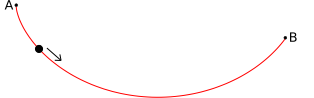
\includegraphics{brachistochrone.png}
\end{center}
}

%-------------------------------------------------------------------------------
%	CHAPTER 6
%-------------------------------------------------------------------------------

\chapter[Euler-Lagrange II]{The Euler-Lagrange equation, II:\\ Constraints}

Imposing constraints works in the infinite-dimensional theory just as well as it does in the finite-dimensional theory using the method of Lagrange multipliers. We will only consider constraints of the form
\[G(y)=\int_a^bM(x,y(x),y'(x))dx=0\]
for some Lagrangian $M(p,q,r)$.

\begin{exm}
Suppose we want to minimise the arc-length of the graph of $y\colon[a,b]\to\RR$ given that the area underneath the graph is equal to $K$. Now
\[A(y)=\int_a^b\sqrt{1+(y')^2}dx\]
is the arc-length and
\[G(y)=\int_a^b\left(y-\frac{K}{b-a}\right)dx\]
measures how far the area underneath the graph is from $K$. We introduce a Lagrange multiplier $\lambda$ and minimise the functional
\[F(y,\lambda)=\int_a^b\left(\sqrt{1+(y')^2}-\lambda\left(y-\frac{K}{b-a}\right)\right)dx.\]
Varying with respect to $\lambda$ gives us the constraint $G(y)=0$ (i.e. the area under the graph of $y$ is $K$) and with respect to $y$ gives the Euler-Lagrange equation
\[-\lambda=\frac{d}{dx}\frac{y'}{\sqrt{1+(y')^2}}\]
so
\[y'=\frac{D-\lambda x}{\sqrt{1-(D-\lambda x)^2}}.\]
Using $D-\lambda x=\sin\theta$ we get $\lambda y+C=\cos\theta$ for some constant $C$, so
\[(\lambda y +C)^2+(D-\lambda x)^2=1\]
and the graph $(x,y(x))$ lies on a circle of radius $1/\lambda$ (it is a segment of circle between $(a,y_a)$ and $(b,y_b)$).

We could also have used Beltrami's identity.
\end{exm}
\begin{exm}[Catenary]
Consider a chain hanging above the $x$-axis with its endpoints fixed at $(a,y_a)$, $(b,y_b)$. It will hang so as to minimise its total potential energy. If the chain is uniform with density $\rho\ kg m^{-1}$ then the segment lying over an infinitesimal segment $dx$ has mass $\rho\sqrt{1+(y')^2}dx$. The potential energy of this segment is $\rho gy\sqrt{1+(y')^2}dx$ so the functional to be minimised is
\[A(y)=\rho g\int_a^by\sqrt{1+(y')^2}dx.\]
However, the chain is inelastic so its length is fixed at $K$ metres
\[G(y)=\int_a^b\left(\sqrt{1+(y')^2}-\frac{K}{b-a}\right)dx=0.\]
The modified functional for the constrained problem is
\[\int_a^b\left(\rho gy\sqrt{1+(y')^2}-\lambda\left(\sqrt{1+(y')^2}-\frac{K}{b-a}\right)\right)dx\]
which has no explicit $x$-dependence, so we will solve this constrained problem using Beltrami's identity.

Beltrami's identity implies
\[\rho gy\sqrt{1+(y')^2}-\lambda\left(\sqrt{1+(y')^2}-\frac{K}{b-a}\right)-y'(\rho gy-\lambda)y'/\sqrt{1+(y')^2}=c\]
for some constant $c$. This gives
\[\rho gy-\lambda=\left(c-\lambda K/(b-a)\right)\sqrt{1+(y')^2}.\]
We define $C:=c-\lambda K/(b-a)$ and we rearrange to get
\[y'=\sqrt{(\rho gy-\lambda)^2/C^2-1}.\]
Substituting $\cosh z=(\rho gy-\lambda)/C$ we integrate and get
\[x=\frac{C}{\rho g}\cosh^{-1}\frac{\rho gy-\lambda}{C}-D\]
or
\[y=\frac{C}{\rho g}\cosh\left(\frac{\rho g}{c}(x+D)\right)+\frac{\lambda}{\rho g}.\]
This curve is called the {\em catenary curve} from the Latin ``catena'' meaning chain. It is the same as the curve whose surface of revolution (catenoid) minimises surface area.
\end{exm}

%-------------------------------------------------------------------------------
%	CHAPTER 7
%-------------------------------------------------------------------------------

\chapter[Euler-Lagrange, III]{The Euler-Lagrange equation, III:\\ More variables}

\section{Vector-valued functions}

We have already seen an example (action of a curve in the plane) where the functions of interest are vector-valued.

\begin{thm}
Let $V$ be the space of functions $\vec{y}\colon [a,b]\to\RR^n$ satisfying the boundary conditions $\vec{y}(a)=\vec{y}_a$ and $\vec{y}(b)=\vec{y}_b$. We will write $\vec{y}(x)$ in coordinates $(y_1(x),\ldots,y_n(x))$. Let $A$ be a functional defined by a Lagrangian $L(p,q_1,\ldots,q_n,r_1,\ldots,r_n)$ by
\[A(\vec{y})=\int_a^bL(x,y_1(x),\ldots,y_n(x),y'_1(x),\ldots,y'_n(x))dx.\]
Let $\vec{\epsilon}(x)$ be a function such that $\vec{\epsilon}(a)=\vec{\epsilon}(b)=0$. Then the G\^{a}teaux derivative of $A$ at $\vec{y}$ in the $\vec{\epsilon}$ direction is
\[d_{\vec{y}}A(\vec{\epsilon})=\sum_{i=1}^n\int_0^1\left(\frac{\partial L}{\partial y_i}-\frac{d}{dx}\frac{\partial L}{\partial y'_i}\right)\epsilon_i(x)dx\]
which vanishes for all $\vec{\epsilon}$ if and only if the $n$ Euler-Lagrange equations hold
\[\frac{\partial L}{\partial y_i}-\frac{d}{dx}\frac{\partial L}{\partial y'_i}=0,\qquad i=1,\ldots,n.\]
\end{thm}
The proof is so similar to the proof for functions $y\colon[a,b]\to\RR$ that I will omit it.

\subsection{Examples}

\begin{exm}[Isoperimetric problem]
Let $\gamma\colon\RR\to\RR^2$ be a curve with coordinates $\gamma(t)=(x(t),y(t))$. We assume that $\gamma$ is a closed curve ($\gamma(t+2\pi)=\gamma(t)$ which is just as good for integrating by parts as assuming $\gamma(0)$ and $\gamma(1)$ are fixed. Suppose that we know it has action $\int_0^1{2\pi}(\dot{x}^2+\dot{y}^2)dt=K$ and we want to maximise the area of the region it bounds.

By Green's theorem, the area of this region $U$ is
\[\int_Udxdy=\int_{\partial U}xdy\]
or
\[\int_0^{2\pi}x(t)\dot{y}(t)dt.\]
Therefore we must find the critical points of the constrained problem
\[\int_0^{2\pi}\left(x\dot{y}-\lambda\left(\dot{x}^2+\dot{y}^2-K/2\pi\right)\right)dt.\]
The two Euler-Lagrange equations are
\begin{align*}
\dot{y}&=\frac{d}{dt}\left(-2\lambda\dot{x}\right)\\
0&=\frac{d}{dt}\left(x-2\lambda\dot{y}\right).
\end{align*}
This gives
\[\ddot{x}=-\dot{y}/2\lambda,\qquad\ddot{y}=\dot{x}/2\lambda.\]
Differentiating again allows us to rearrange and obtain
\[\dddot{y}=-\dot{y}/4\lambda^2,\qquad\dddot{x}=-\dot{x}/4\lambda^2\]
so $\dot{x}$ and $\dot{y}$ obey simple harmonic motion. This means that $t\mapsto(x(t),y(t))$ is a circle.
\end{exm}

\section{Functions of several variables}

Now let $U\subset\RR^m$ be an open subset whose boundary $\partial U$ is smooth. We will consider functions $\phi\colon U\to\RR$ with fixed boundary values; in other words we will fix a function $\phi_0\colon\partial U\to\RR$ and consider functions $\phi$ such that
\[\phi(\vec{x})=\phi_0(\vec{x}),\qquad\vec{x}\in\partial U.\]
Perturbations $\epsilon(\vec{x})$ satisfy $\epsilon(\vec{x})=0$ for $\vec{x}\in\partial U$. Our Lagrangian $L$ will now depend on $\vec{x}=(x_1,\ldots,x_m)$, on $\phi(\vec{x})$ and on the partial derivatives $\partial_i\phi=\frac{\partial \phi}{\partial x_i}$, $i=1,\ldots,m$, that is:
\[A(\vec{y})=\int_UL\left(\vec{x},\phi(\vec{x}),\nabla\phi(\vec{x})\right)dx_1\cdots dx_m\]

\begin{thm}
The G\^{a}teaux derivative of $A$ at $\phi$ in the $\epsilon$-direction is
\[d_{\phi}A(\epsilon)=\int_0^1\left(\frac{\partial L}{\partial \phi}-\sum_{i=1}^m\frac{\partial}{\partial x_i}\frac{\partial L}{\partial(\partial_i\phi)}\right)\epsilon(x)dx\]
which vanishes for all $\epsilon$ if and only if the Euler-Lagrange equation holds
\[\frac{\partial L}{\partial\phi}-\sum_{i=1}^m\frac{\partial}{\partial x_i}\frac{\partial L}{\partial (\partial_i\phi)}=0.\]
\end{thm}
\begin{proof}
Let $t\epsilon$ be a small perturbation of $\phi$. By the chain rule, we have
\[\left.\frac{d}{dt}\right|_{t=0}L(\phi+t\epsilon)=\epsilon\frac{\partial L}{\partial\phi}+\sum_{i=1}^m(\partial_i\epsilon)\frac{\partial L}{\partial(\partial_i\phi)}.\]
Integrating this over $U$ gives the G\^{a}teaux derivative
\[d_{\phi}A(\epsilon)=\int_U\left(\epsilon\frac{\partial L}{\partial\phi}+\sum_{i=1}^m(\partial_i\epsilon)\frac{\partial L}{\partial(\partial_i\phi)}\right)dx_1\cdots dx_m\]
The last term can be written $\nabla\epsilon\cdot\frac{\partial L}{\partial(\nabla\phi)}$ where $\frac{\partial L}{\partial(\nabla\phi)}$ denotes the vector whose $i$th component is $\frac{\partial L}{\partial(\partial_i\phi)}$.

We have
\[\nabla\cdot\left(\epsilon\frac{\partial L}{\partial(\nabla\phi)}\right)=\nabla\epsilon\cdot\frac{\partial L}{\partial(\nabla\phi)}+\epsilon\nabla\cdot\frac{\partial L}{\partial(\nabla\phi)}=\sum_{i=1}^m\left(\partial_i\epsilon\frac{\partial L}{\partial(\partial_i\phi)}+\epsilon\frac{\partial}{\partial x_i}\frac{\partial L}{\partial(\partial_i\phi)}\right).\]
Integrating this over $U$ and applying Stokes's theorem gives
\[\int\nabla\epsilon\cdot\frac{\partial L}{\partial(\nabla\phi)}dx_1\cdots dx_m=-\int_{\partial U}\epsilon\frac{\partial L}{\partial(\nabla\phi)}\cdot\hat{\vec{n}}dS\]
where $\hat{\vec{n}}$ is the outward normal to $\partial U$ and $dS$ is the volume element on $\partial U$. This vanishes because $\epsilon$ vanishes on $\partial U$. Therefore
\[\int_U\nabla\epsilon\cdot\frac{\partial L}{\partial(\nabla\phi)}dx_1\cdots dx_m=-\int_U\epsilon\nabla\cdot\frac{\partial L}{\partial(\nabla\phi)}=-\int_U\sum_{i=1}^m\epsilon\frac{\partial}{\partial x_i}\frac{\partial L}{\partial(\partial_i\phi)}\]
which is the analogue of integration by parts in several variables. This allow us to deduce
\[d_{\phi}A(\epsilon)=\int_U\left(\frac{\partial L}{\partial\phi}-\nabla\cdot\frac{\partial L}{\partial(\nabla\phi)}\right)\epsilon dx_1\cdots dx_m.\]
The fundamental theorem of the calculus of variations in several variables\footnote{This is proved in the same way as the one-variable case but using a bump-function in several variables - this can be taken to be the usual bump function applied to the radius $\sqrt{\sum_{i=1}^mx_i^2}$.} states that this vanishes for all $\epsilon$ if and only if
\[\frac{\partial L}{\partial\phi}-\nabla\cdot\frac{\partial L}{\partial(\nabla\phi)}=0.\]
Unwinding the definition of $\partial L/\partial(\nabla\phi)$ gives the formulae in the statement of the theorem.
\end{proof}
\begin{rmk}
The Euler-Lagrange equation is now a second-order \emph{partial} differential equation.
\end{rmk}

\subsection{Examples}

\begin{exm}
Consider $U=[0,1]^2$, the square, and functions $\phi$ with fixed boundary values
\begin{align*}
\phi(x,0)&=\phi_0(x,0),&\phi(x,1)&=\phi_0(x,1),\\
\phi(0,y)&=\phi_0(0,y),&\phi(1,y)&=\phi_0(1,y).
\end{align*}
We will try to minimise the functional
\[A(\phi)=\int_0^1\int_0^1\left(\left(\frac{\partial\phi}{\partial x}\right)^2+\left(\frac{\partial\phi}{\partial y}\right)^2\right)dx dy.\]
We can think of this functional as the total gradient $\int|\nabla\phi|^2dxdy$ of a temperature distribution $\phi$ on $U$. Since heat flows to minimise a gradient, a minimiser for this functional will be a steady-state temperature distribution on the square.

We have
\[\frac{\partial L}{\partial \phi}=0\qquad\frac{\partial L}{\partial(\partial_x\phi)}=2\partial_x\phi,\qquad\frac{\partial L}{\partial(\partial_y\phi)}=2\partial_y\phi\]
so the Euler-Lagrange equation is
\[\frac{\partial^2\phi}{\partial x^2}+\frac{\partial^2\phi}{\partial y^2}=0.\]
This is called Laplace's equation and will be important later in the course.
\end{exm}
\begin{exm}
Now let us use the functional
\[A(\phi)=\int_U\sqrt{1+(\partial_x\phi)^2+(\partial_y\phi)^2}dx dy.\]
This measures the area of the graph\footnote{To see this, note that the two vectors $(1,0,\partial_x\phi)$ and $(0,1,\partial_y\phi)$ are tangent to the graph of $\phi$ and they span a parallelogram with area $\sqrt{1+(\partial_x\phi)^2+(\partial_y\phi)^2}$. The infinitesimal area element living over $dx dy$ is therefore an infinitesimal parallelogram of area $\sqrt{1+(\partial_x\phi)^2+(\partial_y\phi)^2}dxdy$.} of $\phi$. The Euler-Lagrange equation is 
\[\frac{\partial L}{\partial\phi}=\frac{\partial}{\partial x}\frac{\partial L}{\partial\phi_x}+\frac{\partial}{\partial y}\frac{\partial L}{\partial\phi_y}\]
and in this case
\[L=\sqrt{1+\phi_x^2+\phi_y^2}\]
so
\begin{align*}
0&=\frac{\partial}{\partial x}\frac{\phi_x}{\sqrt{1+|\nabla\phi|^2}}+\frac{\partial}{\partial y}\frac{\phi_y}{\sqrt{1+|\nabla\phi|^2}}\\
&=\frac{\Delta\phi}{\sqrt{1+|\nabla\phi|^2|}}-\frac{\phi_x(\phi_x\phi_{xx}+\phi_y\phi_{yy})+\phi_y(\phi_y\phi_{yy}+\phi_x\phi_{xy})}{(1+|\nabla\phi|^2)^{3/2}}\\
&=\frac{1}{(1+|\nabla\phi|^2)^{3/2}}\left(\phi_{xx}(1+\phi_y^2)+\phi_{yy}(1+\phi_x^2)-2\phi_x\phi_y\phi_{xy}\right)
\end{align*}
(remember that $\nabla\phi=(\phi_x,\phi_y)$ and $\Delta\phi=\phi_{xx}+\phi_{yy}$). This gives us the equation for a {\em minimal surface}:
\[\frac{\partial^2\phi}{\partial x^2}\left(1+\left(\frac{\partial\phi}{\partial y}\right)^2\right)+\frac{\partial^2\phi}{\partial y^2}\left(1+\left(\frac{\partial\phi}{\partial x}\right)^2\right)=2\frac{\partial\phi}{\partial x}\frac{\partial\phi}{\partial y}\frac{\partial^2\phi}{\partial x\partial y}.\]
\end{exm}

%%% Local Variables: 
%%% mode: latex
%%% TeX-master: "notes"
%%% End: 

\part{Partial differential equations}

%\include{pde}

%-------------------------------------------------------------------------------

% CHAPTER 12

%-------------------------------------------------------------------------------

\chapter[Method of characteristics, I]{Method of characteristics, I: Linear case}

Over the next two chapters we will develop a method for solving first order PDEs called the method of characteristics. In this chapter we will restrict attention to inhomogeneous linear equations (first with constant coefficients, then with nonconstant coefficients) where the method of characteristics boils down to finding a sensible change of coordinates after which the PDE looks much simpler.

\section{Linear change of coordinates}\label{sct:linearcoord}

Occasionally, for very simple PDEs, one can change coordinates and turn them into PDEs we already know how to solve.

\subsection{Examples}
\begin{exm}
Consider the PDE for $\phi(x,y)$:
\[\frac{\partial\phi}{\partial x}=0.\]
This says $\phi$ is constant in the $x$-direction, so $\phi$ is a function of $y$ alone. Any function of $y$ is a solution, i.e. $\phi(x,y)=C(y)$ where $C$ is an arbitrary function.
\end{exm}
\begin{exm}
Consider the PDE for $\phi(x,y)$:
\[\frac{\partial\phi}{\partial x}-\frac{\partial\phi}{\partial y}=0.\]
The expression on the left-hand side looks like the expression
\[\pd{\phi}{u}=\pd{x}{u}\pd{\phi}{x}+\pd{y}{u}\pd{\phi}{y}\]
coming from the chain rule, provided we pick
\[\pd{x}{u}=1,\qquad\pd{y}{u}=-1.\]
So let's change to a new (linear) system of coordinates $(u,v)$ satisfying
\[\pd{x}{u}=1,\qquad\pd{y}{u}=-1.\]
For example we could take
\[\twob{x}{y}=\matr{1}{0}{-1}{1}\twob{u}{v}\]
or
\[\twob{x}{y}=\matr{1}{7}{-1}{0}\twob{u}{v}.\]
The only conditions for this to define a suitable coordinate change are:
\begin{itemize}
\item that the first column is given by $1$ and $-1$ (the coefficients of $\pd{\phi}{x}$ and $\pd{\phi}{y}$ in the equation),
\item that the matrix is invertible.
\end{itemize}
Let's use
\[\twob{x}{y}=\matr{1}{0}{-1}{1}\twob{u}{v}\]
whose inverse is
\[\twob{u}{v}=\matr{1}{0}{1}{1}\twob{x}{y}\]
With respect to the new basis, the chain rule tells us that
\begin{align*}
\pd{\phi}{u}&=\pd{x}{u}\pd{\phi}{x}+\pd{y}{u}\pd{\phi}{y}\\
            &=\pd{\phi}{x}-\pd{\phi}{y}\\
            &=0\mbox{ (by our equation)}
\end{align*}
so the general solution to the equation is $\phi(u,v)=C(v)$. In terms of the original basis this is $\phi(x,y)=C(x+y)$. So any function of $v=x+y$ is a solution. For example $\sin(x+y)$, $e^{7(x+y)}$,...
\end{exm}
\begin{exm}
Consider the PDE for $\phi(x,y)$:
\[\frac{\partial\phi}{\partial x}-\frac{\partial\phi}{\partial y}=x.\]
If we make the same change of coordinates as before,
\[\twob{x}{y}=\matr{1}{0}{-1}{1}\twob{u}{v},\qquad \twob{u}{v}=\matr{1}{0}{1}{1}\twob{x}{y}\]
this equation becomes
\begin{align*}
\pd{\phi}{u}&=\pd{x}{u}\pd{\phi}{x}+\pd{y}{u}\pd{\phi}{y}\\
            &=\pd{\phi}{x}-\pd{\phi}{y}\\
            &=x\mbox{ (by our equation)}\\
            &=u\mbox{ (by our coordinate change).}
\end{align*}
We can integrate this and get
\[\phi(x,y)=\frac{1}{2}u^2+C(v)\]
where $C(v)$ is an arbitrary function of $v=x+y$. Translating back into our original coordinates we get
\[\phi(x,y)=\frac{x^2}{2}+C\left(x+y\right).\]
\end{exm}
\subsection{In general}
This trick works with any PDE for $\phi(x_1,\ldots,x_n)$ of the form
\[\sum_{i=1}^nA_i\frac{\partial\phi}{\partial x_i}=0\]
In new coordinates $(u_1,\ldots,u_n)$, we have
\[\pd{\phi}{u_1}=\sum_{i=1}^n\pd{x_i}{u_1}\pd{\phi}{x_i}\]
so $\pd{\phi}{u}=\sum A_i\pd{\phi}{x_i}$ if $\pd{x_i}{u_1}=A_i$. A suitable linear change of coordinates is therefore
\[\left(\begin{array}{c}
x_1\\
\vdots\\
x_n
\end{array}\right)=\left(\begin{array}{ccc}A_1 & \star & \star\\
\vdots & \vdots & \vdots\\
A_n & \star & \star\end{array}\right)\left(\begin{array}{c}u_1\\ \vdots\\ u_n\end{array}\right)\]
where the stars can be anything, provided the matrix is invertible. With this change of coordinates, the chain rule tells us that
\[\pd{\phi}{u}=\sum A_i\pd{\phi}{x_i}\]
so the solution to the equation $\sum A_i\pd{\phi}{x_i}=0$ is
\[C(u_2,\ldots,u_n)\]
for an arbitrary function $C$.

\begin{exm}
Consider the equation
\[\pd{\phi}{x}+2\pd{\phi}{y}=\sin y.\]
Use the coordinate change
\[\twob{x}{y}=\matr{1}{0}{2}{1}\twob{u}{v}\]
whose inverse is
\[\twob{u}{v}=\matr{1}{0}{-2}{1}\twob{x}{y}.\]
The chain rule tells us that
\begin{align*}
\pd{\phi}{u}&=\pd{x}{u}\pd{\phi}{x}+\pd{y}{u}\pd{\phi}{y}\\
            &=\pd{\phi}{x}+2\pd{\phi}{y}\\
            &=\sin y\\
            &=\sin(2u+v).
\end{align*}
Then, fixing $v$ and integrating with respect to $u$, we get
\[\phi(u,v)=-\frac{1}{2}\cos(2u+v)+C(v)\]
or
\[\phi(x,y)=-\frac{1}{2}\cos y+C(y-2x).\]
\end{exm}

\subsection{Boundary conditions}

If we want to fix the arbitrary function $C$ then we need more information.

\begin{exm}
{\bf Solve the equation
\[\pd{\phi}{x}+2\pd{\phi}{y}=\sin y\]
subject to the boundary condition $\phi(s,0)=s^2$.}

We have already seen that the general solution to this equation is $\phi(x,y)=-\frac{1}{2}\cos y+C(y-2x)$. If we substitute this into the boundary condition then we get
\[s^2=-\frac{1}{2}\cos(0)+C(0-2s)\]
which means
\[C(-2s)=s^2+\frac{1}{2}.\]
Substituting $w=-2s$ ($s=-w/2$) gives
\[C(w)=\frac{w^2}{4}+\frac{1}{2}.\]
\end{exm}

\section{Nonlinear change of coordinates}

We have only allowed ourselves to change coordinates by a linear transformation. What kind of equations do we get if we make more interesting coordinate changes?

\subsection{An elementary example}

\begin{exm}
Use plane polar coordinates:
\begin{align*}
x&=r\cos\theta\\
y&=r\sin\theta.
\end{align*}
By the chain rule we have
\begin{align*}
\frac{\partial\phi}{\partial r}&=\frac{\partial\phi}{\partial x}\frac{\partial x}{\partial r}+\frac{\partial\phi}{\partial y}\frac{\partial y}{\partial r}\\
&=\frac{x}{r}\frac{\partial\phi}{\partial x}+\frac{y}{r}\frac{\partial y}{\partial r}
\end{align*}
In particular, the equation
\[\frac{\partial\phi}{\partial r}=0\]
becomes (after multiplying out by $r$)
\begin{equation}\label{eqn-radial-pde-exm}x\frac{\partial\phi}{\partial x}+y\frac{\partial\phi}{\partial y}=0.\end{equation}
In particular, the solutions to Equation \eqref{eqn-radial-pde-exm} are just functions of $\theta=\tan^{-1}(y/x)$. For instance, $\tan(\theta)=y/x$ is a solution (away from $x=0$) or $\cos\theta=x/\sqrt{x^2+y^2}$ is a solution. (Check them!)
\end{exm}

\subsection{Characteristic vector field}

\begin{lma}\label{lma:chain}
Given an expression of the form
\[\sum_{i=1}^nA_i(x_1,\ldots,x_n)\frac{\partial\phi}{\partial x_i},\]
suppose that we can find coordinates $(u_1,\ldots,u_n)$ such that
\[\pd{x_i}{u_1}=A_i(x_1,\ldots,x_n).\]
Then
\[\pd{\phi}{u}=\sum_{i=1}^nA_i(\vec{x})\pd{\phi}{x_i}.\]
\end{lma}
\begin{proof}
This is immediate from the chain rule:
\[\pd{\phi}{u}=\sum_{i=1}^n\pd{x_i}{u_1}\pd{\phi}{x_i}=\sum_{i=1}^nA_i(\vec{x})\pd{\phi}{x_i}.\]
\end{proof}

In fact we can always find suitable coordinates, at least locally. So how do we solve the equations
\[\pd{x_i}{u_1}=A_i(x_1,\ldots,x_n)?\]

\begin{exm}
Consider the equation $x\pd{\phi}{x}+y\pd{\phi}{y}=0$. We want to solve
\[\twob{\pd{x}{u}}{\pd{y}{u}}=\twob{x}{y}.\]
For simplicity, let's write this as
\[\twob{\dot{x}}{\dot{y}}=\twob{x}{y}.\]
The solution is $x=Ae^u$, $y=Be^u$. We want to think of these two equations as giving a coordinate transformation, but we have three new coordinates $u,A,B$, so this doesn't quite make sense yet. Let us make an arbitrary choice: set $A=1$ and take our new coordinates to be $u$ and $v=A$. That is:
\[x=e^u,\qquad y=ve^u.\]
The inverse of this coordinate transformation is
\[u=\ln x,\qquad v=y/x.\]
This arbitrary choice is completely analogous to the way we could choose our matrix entries freely in Section \ref{sct:linearcoord}. With these new coordinates, we have
\[x\pd{\phi}{x}+y\pd{\phi}{y}=\pd{\phi}{u}\]
by Lemma \ref{lma:chain}. Therefore the equation is $\pd{\phi}{u}=0$ and the solution is $\phi(u,v)=C(v)$ (where $C$ is an arbitrary function). Substituting our expression $v=y/x$ we get
\[\phi(x,y)=C(y/x).\]
\end{exm}

\begin{dfn}
Consider an equation of the form $A(x,y)\pd{\phi}{x}+B(x,y)\pd{\phi}{y}+C(x,y)\phi+D(x,y)=0$ (``inhomogeneous linear''). The vector field
\[\twob{A(x,y)}{B(x,y)}\]
is called the characteristic vector field. The differential equations
\[\twob{\dot{x}}{\dot{y}}=\twob{A(x,y)}{B(x,y)}\]
are called the characteristic equations and a curve $(x(u),y(u))$ satisfying the characteristic equations is called a characteristic curve (it is always tangent to the characteristic vector field). This method for solving first order PDEs is called the {\em method of characteristics}.
\end{dfn}

\begin{rmk}
In general, if you have a vector field $(A(x,y),B(x,y))$ and a curve satisfying
\[\dot{x}=A(x,y),\qquad \dot{y}=B(x,y)\]
then the curve is called an {\em integral curve} (it's found by integrating (i.e. solving) these differential equations). I may occasionally slip and use this terminology, so it's best that you're aware of it.
\end{rmk}

\begin{exm}
Consider the equation
\[-y\pd{\phi}{x}+x\pd{\phi}{y}=0.\]
The characteristic vector field is $(-y,x)$ and the characteristic equations are
\[\dot{x}=-y,\qquad\dot{y}=x.\]
Differentiating again we get $\ddot{x}=-x$, so $x=A\cos u+B\sin u$ and $y=-\dot{x}=A\sin u-B\cos u$. Let us pick $B=0$ and $v=A$. Now we have
\[(x,y)=(v\cos u,v\sin u).\]
The inverse coordinate transform is
\[v=\sqrt{x^2+y^2},\qquad u=\tan^{-1}(y/x).\]
The equation becomes $\pd{\phi}{u}=0$ which has solution $C(v)=C(\sqrt{x^2+y^2})$.
\end{exm}

{
\begin{center}
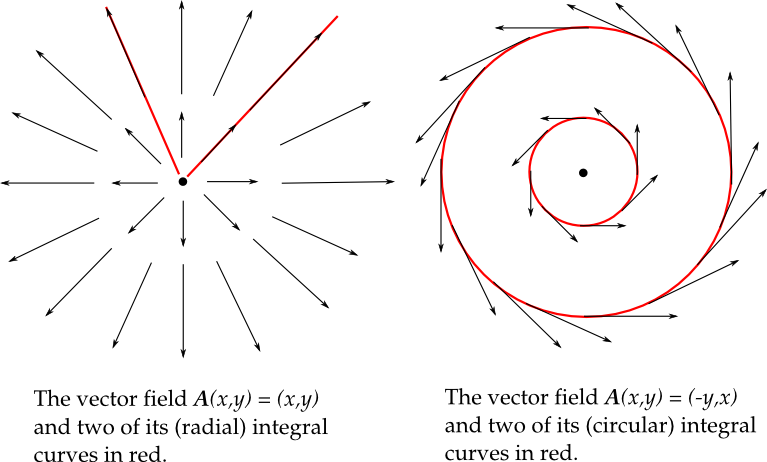
\includegraphics[width=400px]{integral-curves.png}
\end{center}
}

\begin{exm}
Consider the equation
\begin{equation}\label{eqn-pde-characteristic-exm}x\frac{\partial\phi}{\partial x}-\frac{\partial\phi}{\partial y}=0.\end{equation}
The characteristic vector field in this equation is $(x,-1)$. The characteristic curves $(x(u),y(u))$ are solutions to
\[\dot{x}=x,\ \dot{y}=-1.\]

{
\begin{center}
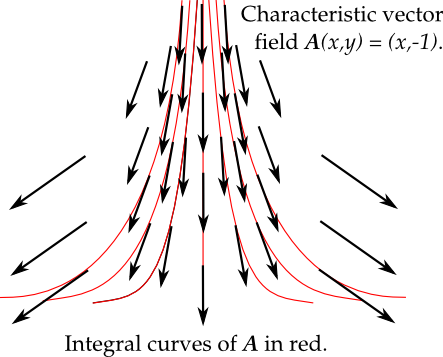
\includegraphics[width=250px]{characteristics2.png}
\end{center}
}

These equations have solution
\[x=Ae^u,\qquad y=B-u\]
Pick $B=0$ and $v=A$. The new coordinates are therefore
\begin{align*}
x&=ve^u,&y&=-u\\
u&=-y,&v&=xe^y.
\end{align*}

{
\begin{center}
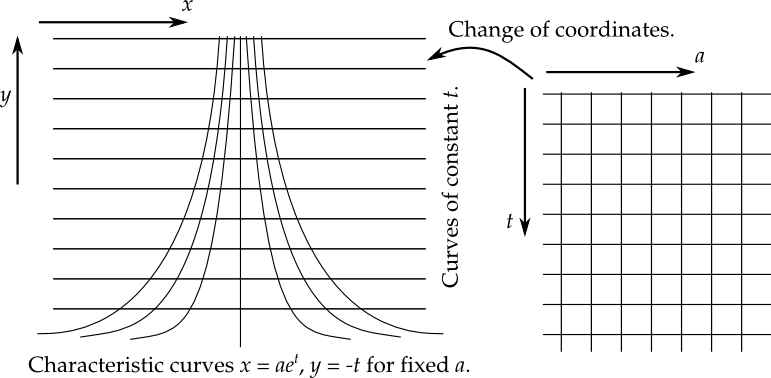
\includegraphics[width=400px]{characteristics1.png}
\end{center}
}

Lemma \ref{lma:chain} tells us that
\[\pd{\phi}{u}=x\pd{\phi}{x}-\pd{\phi}{y}\]
so Equation \eqref{eqn-pde-characteristic-exm} becomes $\pd{\phi}{u}=0$ and has solution $\phi(u,v)=C(v)$. In other words, $\phi(x,y)=C(xe^y)$.
\end{exm}

\begin{rmk}\label{rmk:bequalszero}
How did we make this choice $B=0$? Since $y=B-u$ we could always achieve $B=0$ by translating in the $t$ coordinate, that is using the new $u$-coordinate $\tilde{u}=u-B$, in terms of which $y=-\tilde{u}$. If we had picked $A=0$, $B=v$ then the corresponding ``change of coordinates'' would have been $x=0$, $y=v-u$, which isn't really a change of coordinates because you can never express points with $x\neq 0$ in terms of $u$ and $v$.
\end{rmk}

\begin{exm}
To illustrate what happens for different choices, let's work through what would have happened if we had picked $A=1$, $B=v$ in the previous example. The corresponding change of coordinates would have been $x=e^u$, $y=v-u$. The equation has solution $\tilde{C}(v)=\tilde{C}(y+\ln x)$. This looks different from the previous answer, but notice that $y+\ln x=\ln(xe^y)$, so they're really the same solution in disguise! In particular, if you take $\tilde{C}(v)=C(e^v)$ then you really have the same solution. Going backwards, $C(v)=\tilde{C}(\ln v)$ gives a correspondence between solutions, but notice that this only makes sense when $v>0$. Indeed, if you look at the coordinates defined by $x=e^u$, $y=v-u$, you can see that these coordinates only cover the region $x>0$.
\end{exm}

\begin{rmk}
In summary, this solution is just as valid as the previous solution, but you should be careful to point out that the solution is only defined on the region $x>0$ of the plane. In general, choosing which constants of integration to use as coordinates requires some thought specific to the problem at hand. You may need to use different choices to cover different regions of the plane. You will build up a feeling for which choices are sensible by working with examples. Sometimes you can say ``without loss of generality we can set $B=0$'' (or something like that) as in Remark \ref{rmk:bequalszero} but often you just have to make a judicious choice.
\end{rmk}

\section{More examples}

\begin{exm}
Consider the PDE for $\phi(x,y)$:
\[\frac{1}{x}\frac{\partial\phi}{\partial x}-y\frac{\partial\phi}{\partial y}=0.\]
The characteristic vector field is $(1/x,-y)$ so the characteristic curves satisfy
\[\dot{x}=1/x,\ \dot{y}=-y.\]
The first equation can be rearranged as $x\dot{x}=1$ or $\frac{1}{2}\pd{x^2}{u}=1$ so $x=\sqrt{2u+A}$. The second equation has solution $y=Be^{-u}$. We can reparametrise $u$ to $\tilde{u}=u-A/2$ so that without loss of generality $A=0$. Our new coordinates are therefore $(u,v)$ where $u=x^2/2$ and $v=B=ye^u=ye^{x^2/2}$. In these new coordinates the PDE becomes
\[\frac{\partial\phi}{\partial u}=0\]
so solutions to the PDE are just arbitrary functions of $v=ye^{x^2/2}$.
\end{exm}
\begin{exm}
Consider the PDE for $\phi(x,y)$:
\[\frac{1}{x}\frac{\partial\phi}{\partial x}-y\frac{\partial\phi}{\partial y}=y.\]
The characteristic vector field and characteristic curves are the same as in the previous example so our new coordinates are again $(u,v)=(x^2/2,ye^{x^2/2})$. In these new coordinates the equation becomes
\[\frac{\partial\phi}{\partial t}=y=ve^{-u}.\]
Integrating this we get
\[\phi(u,v)=-ve^{-u}+C(v)\]
for some arbitrary function $C$. In other words, returning to our original coordinates,
\[\phi(x,y)=-y+C(ye^{x^2/2}).\]
\end{exm}
\begin{exm}
Consider the PDE for $\phi(x,y)$:
\[\frac{\partial\phi}{\partial x}+2x\frac{\partial\phi}{\partial y}=1.\]
The characteristic vector field is $(1,2x)$ so the characteristic curves satisfy
\[\dot{x}=1,\ \dot{y}=2x,\]
thus $x=u+A$ and $y=(u+A)^2+B$. Reparametrising so that $A=0$ and setting $v=B$, we get $(x,y)=(u,u^2vB)$ or $(u,v)=(x,y-x^2)$ as our change of coordinates. The PDE becomes
\[\frac{\partial\phi}{\partial u}=1\]
so $\phi(u,v)=u+C(v)$ for some arbitrary function $C$. In other words,
\[\phi(x,y)=x+C(y-x^2).\]
\end{exm}
\begin{exm}
Consider the PDE for $\phi(x,y)$:
\[y\frac{\partial\phi}{\partial x}+x\frac{\partial\phi}{\partial y}=0.\]
The characteristic vector field is $(y,x)$ so the characteristic curves satisfy
\[\dot{x}=y,\ \dot{y}=x\]
Differentiating with respect to $u$ again we get $\ddot{x}=x$ so $x=Ae^u+Be^{-u}$. Since $y=\dot{x}$ we have $y=Ae^u-Be^{-u}$. If we want to understand these curves geometrically, notice that $x^2-y^2=4AB$ so if $AB$ is fixed then the characteristic curves are hyperbolae.

There is no single choice like $A=0$ or $B=0$ which will give us a good coordinate system everywhere. If there were we would be able to change coordinates and make the hyperbolae look like a family of parallel lines, but the hyperbola $x^2-y^2=0$ consists of two straight lines intersecting at a point, which can never be made to look like a single straight line!

If we pick $A=0$ or $B=0$ then we can only ever hope for our coordinates to to cover points on the hyperbola $x^2-y^2=4ab=0$, so we should pick a nonzero value for $A$ or $B$.

We will try fixing $B=1$, $A=v$, so $x=ve^u+e^{-u}$ and $y=ve^u-e^{-u}$. As expected, this choice of coordinates does not cover the whole plane: $x-y=2e^{-u}$ is always positive so we can only cover the part of the plane to the right of the line $y=x$. But at least that is a large open subset. With this choice, $u=-\ln\left(\tfrac{1}{2}(x-y)\right)$ and $v=(x^2-y^2)/4$. The PDE becomes
\[\frac{\partial\phi}{\partial u}=0\]
and the solution is $\phi(u,v)=C(v)$, that is
\[\phi(x,y)=C((x^2-y^2)/4).\]
If you try $B=-1$ you will get coordinates to cover the other half of the plane and if you choose $A=\pm 1$ you will get coordinates to cover the two halves of the plane separated by the line $y=-x$. However, these all lead to the same answer: $\phi(x,y)$ is an arbitrary function of $\tfrac{1}{4}(x^2-y^2)$.
\end{exm}

\begin{exm}
{\bf Consider the PDE for $\phi(x,y)$:
\[y\frac{\partial\phi}{\partial x}+x\frac{\partial\phi}{\partial y}+xy\phi=0\]
and try to solve it with the boundary condition $\phi(s,1)=\sin s$.}

This looks a little different because of the $xy\phi$ term, but it is amenable to the same method of solution. The characteristic vector field is the same as in the previous example and we choose the coordinates
\begin{align*}
u&=-\ln\left(\tfrac{1}{2}(x-y)\right) & x&=ve^u+e^{-u}\\
v&=(x^2-y^2)/4&y&=ve^u-e^{-u}.
\end{align*}
The PDE becomes
\[\frac{\partial\phi}{\partial u}=-xy\phi=-\left(v^2e^{2u}-e^{-2u}\right)\phi\]
that is
\[\frac{\partial}{\partial u}\ln\phi=-v^2e^{2u}+e^{-2u}\]
and we integrate up to get
\[\ln\phi=-\frac{1}{2}\left(v^2e^{2u}+e^{-2u}\right)+C(v)\]
or
\[\phi(x,y)=\exp\left(-\frac{x^2+y^2}{4}\right)\tilde{C}\left(\tfrac{1}{4}(x^2-y^2)\right)\]
where $\tilde{C}$ is an arbitrary function.

The boundary condition tell us that $\phi(s,1)=\sin s$ so
\[\exp(-(s^2+1)/4)\tilde{C}((s^2-1)/4)=\sin s\]
which means
\[\tilde{C}((s^2-1)/4)=\exp((s^2+1)/4)\sin s.\]
Substituting $w=(s^2-1)/4$ ($s=\sqrt{4w+1}$, $(s^2+1)/4=w+1/2$) gives
\[\tilde{C}(w)=\exp(w+1/2)\sin\sqrt{4w+1}.\]
Therefore the relevant solution is
\[\exp(-(x^2+y^2)/4)\exp\left(\tfrac{1}{4}(x^2-y^2)+\tfrac{1}{2}\right)\sin\sqrt{x^2-y^2+1}.\]
\end{exm}

\chapter[Method of characteristics, II]{Method of characteristics, II: Quasilinear case}

We now consider first order quasilinear equations
\begin{equation}\label{eqn-quasilinear}A(x,y,\phi)\frac{\partial\phi}{\partial x}+B(x,y,\phi)\frac{\partial\phi}{\partial y}+C(x,y,\phi)=0\end{equation}
which are more complicated because all the coefficients are allowed to depend on $\phi$. For notational simplicity, we will only consider the case where $\phi(x,y)$ is a function of two variables.
\begin{dfn}
If $\phi$ is a solution of \eqref{eqn-quasilinear} defined for $(x,y)$ in some open set $U\subset\RR^2$ then the graph of $\phi$ is the set of points
\[\{(x,y,\phi(x,y))\ :\ (x,y)\in U\}\]
in other words, the surface in $\RR^3=\{(x,y,z)\ :\ x,y,z,\in\RR\}$ cut out by the equation $z=\phi(x,y)$.
\end{dfn}
We will look for a solution by constructing its graph.


\section{Characteristic vector field}

\begin{dfn}
The {\em characteristic vector field} of
\[A(x,y,\phi)\frac{\partial\phi}{\partial x}+B(x,y,\phi)\frac{\partial\phi}{\partial y}+C(x,y,\phi)=0\]
is
\[(A(x,y,z),B(x,y,z),-C(x,y,z)).\]
This is now a vector field in $\RR^3$ (coordinates $x,y,z$). A {\em characteristic curve} is a solution
\[(x(t),y(t),z(t))\]
to
\begin{align*}
\frac{dx}{dt}&=A(x(t),y(t),z(t))\\
\frac{dy}{dt}&=B(x(t),y(t),z(t))\\
\frac{dz}{dt}&=-C(x(t),y(t),z(t)).
\end{align*}
\end{dfn}

\begin{dfn}
A one-parameter family of characteristic curves is a smooth map
\[\mathbf{R}^2\supset U\ni(s,t)\mapsto(x(s,t),y(s,t),z(s,t))\in\RR^3\]
where, for fixed $s_0$, each curve $(x(s_0,t),y(s_0,t),z(s_0,t))$ is a characteristic curve. The image of this map is a surface in $\RR^3$. We call this a {\em solution surface} for \eqref{eqn-quasilinear} (see Theorem \ref{thm:solsurf} below to find out why).
\end{dfn}

\begin{dfn}
A surface in $\RR^3$ is a {\em graph} if it is of the form $z=\phi(x,y)$ for some function $\phi$. For example,
\begin{itemize}
\item $\{y=0\}\subset\RR^3$ is not a graph: it is vertical;
\item $\{z^2=1\}\subset\RR^3$ is not a graph: it is the union of two graphs $\{z=1\}$ and $\{z=-1\}$;
\item $\{z^2=x\}\subset\RR^3$ is not a graph: it is the union of two graphs locally, $z=\sqrt{x}$ and $z=-\sqrt{x}$ defined over the half-plane $\{x\geq 0\}\subset\RR^2$. These graphs meet along the line $x=z=0$. Over this line the solution surface becomes vertical (i.e. it has a vertical tangency) which precludes it from being a graph there.
\end{itemize}
\end{dfn}

\begin{thm}\label{thm:solsurf}
Let $(s,t)\mapsto(x_s(t),y_s(t),z_s(t))$ be a solution surface which is (at least locally) the graph of a function $\phi$. Then $\phi$ is a solution of \eqref{eqn-quasilinear}.
\end{thm}
\begin{proof}
Since the surface is a graph we have
\[z_s(t)=\phi(x_s(t),y_s(t)).\]
Fix $s$ and differentiate this with respect to $t$. The chain rule gives
\[\frac{dz_s(t)}{dt}=\frac{\partial\phi}{\partial x}\frac{dx_s}{dt}+\frac{\partial\phi}{\partial y}\frac{dy_s}{dt}\]
and since the solution surface is a one-parameter family of characteristic curves,
\begin{align*}
\frac{dx_s}{dt}&=A(x_s(t),y_s(t),z_s(t))\\
\frac{dy_s}{dt}&=B(x_s(t),y_s(t),z_s(t))\\
\frac{dz_s}{dt}&=-C(x_s(t),y_s(t),z_s(t)).
\end{align*}
Therefore we have
\[-C=A\partial\phi/\partial x+B\partial\phi/\partial y\]
as required.
\end{proof}
\begin{thm}
If $\phi$ is a solution to \eqref{eqn-quasilinear} then its graph is a solution surface (i.e. its graph is traced out by a one-parameter family of characteristic curves).
\end{thm}
\begin{proof}
Consider the equations
\[\dot{x}(t)=A(x(t),y(t),\phi(x(t),y(t))),\qquad\dot{y}(t)=B(x(t),y(t),\phi(x(t),y(t)))\]
for a curve $t\mapsto(x(t),y(t))$ in the plane. We can solve these ordinary differential equations to find a curve in the plane through any given point. Living over this curve there is another curve inside the graph of $\phi$
\[t\mapsto(x(t),y(t),z(t)=\phi(x(t),y(t)))\]
We claim that this is a characteristic curve. Indeed if we differentiate $\phi(x(t),y(t))$ with respect to $t$ using the chain rule we get
\[\frac{d(\phi(x(t),y(t)))}{dt}=\frac{\partial\phi}{\partial x}\dot{x}+\frac{\partial\phi}{\partial y}\dot{y}\]
or
\[\dot{z}=A\partial\phi/\partial x+B\partial\phi/\partial y=-C.\]
This shows that through every point of the graph of $\phi$ there passes a characteristic curve which is completely contained in the graph, as required.
\end{proof}

\section{Example: A linear equation!}

We can, of course, apply these methods to simpler, linear equations. Take the equation $\pd{\phi}{x}=0$ with the initial condition $\phi(0,s)=s$. We know that the general solution is $C(y)$ for some function $C$ and the initial condition implies $C(s)=s$, so the solution is $\phi(x,y)=y$. Let's solve it using the quaslinear method of characteristics instead. The characteristic equations are
\begin{align*}
\dot{x}&=1\\
\dot{y}&=0\\
\dot{z}=0
\end{align*}
so
\[x=t+a,\ y=b,\ z=c\]
for some constants $a,b,c$. Fixing $a,b,c$ and letting $t$ vary gives the characteristic curves in $\RR^3$: these are just straight lines parallel to the $x$-axis! The graph of our solution is a surface swept out by a one-parameter family of these parallel lines. The fact that the lines are parallel to the $x$-axis means that the resulting graph surface will be flat in the $x$-direction, ence $\pd{\phi}{x}=0$.

We pick the one-parameter family using the initial condition $\phi(0,s)=s$ at $t=0$. This tells us that
\begin{align*}
0=x&=0+a\\
s=y&=b\\
s=z&=c
\end{align*}
so $a=0$, $b=s$, $c=s$. For each value of $s$ we get a characteristic curve
\[t\mapsto (t,s,s)\]
in $(x,y,z)$-space and these trace out the surface
\[(x(s,t),y(s,t),z(s,t))=(t,s,s)\]
(considered as a parametric surface in $\RR^3$). This is supposed to be the graph of our solution $\phi$, and we can find $\phi$ by expressing the $z$-coordinate ($s$) in terms of the $x$ and $y$ coordinates (respectively $t$ and $s$): clearly $z=y$, so the solution is $\phi(x,y)=y$.

\begin{figure}
\begin{center}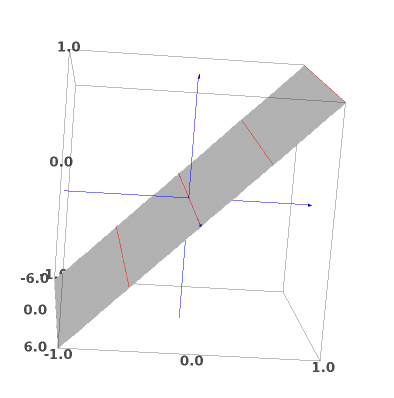
\includegraphics[width=200pt]{qcharacteristic6.png}\end{center}
\caption{The red curves are the characteristic curves parallel to the $x$-axis. The grey surface is the surface traced out by the characteristic curves passing through the initial condition $\phi(0,s)=s$. The initial condition is saying ``pick those characteristic curves which intersect the $x=0$ plane (i.e. the $(y,z)$-plane) at points $y=z$'' which is why the grey surface intersects the $(y,z)$-plane along the diagonal line $y=z$.}
\end{figure}

\section{Example: Burgers's equation}

\begin{exm}\label{exm-burgers-1}
{\bf Solve the equation
\[\frac{\partial\phi}{\partial x}+\phi\frac{\partial\phi}{\partial y}\]
subject to the initial condition $\phi(0,s)=s$.}

We will worry about the initial condition later. This equation has $A(x,y,z)=1$, $B(x,y,z)=z$ and $C(x,y,z)=0$. The characteristic vector field is
\[\left(\begin{array}{c}1\\ z\\ 0\end{array}\right)\]
so a characteristic curve $(x(t),y(t),z(t))$ satisfies
\[\dot{x}=1,\ \dot{y}=z,\ \dot{z}=0.\]
We can solve this and we get
\[z=a,\ y=at+b,\ x=t+c\]
for constants $a,b,c$. For each fixed $a,b,c$ we get a characteristic curve which is a straight line at constant height $a$, with slope $a$ when considered in the $(x,y)$-plane. To get a solution surface we need to pick a one-parameter family of these curves, i.e. we need give $a,b,c$ in terms of a single parameter $s$.

The specification of an initial condition cuts down the amount of choice. In this case the initial condition is $\phi(0,s)=s$. At this is an initial condition, we will impose it at $t=0$ and use it to determine how $a$, $b$ and $c$ depend on $s$. We know that $x=t+c$, $y=at+b$ and $z=a$. Imposing the initial condition means substituting $t=0$, $x=0$, $y=s$ and $z=s$, then solving for $a,b,c$ in terms of $s$. This gives $c=0$ and $a=b=s$. In other words, if we look at the piece of the solution surface living over the line $x=0$ we get a path $s\mapsto(0,s,s)$ in 3-dimensional space which intersects each characteristic curve at the point $t=0$. We call the corresponding characteristic curve $(x(s,t),y(s,t),z(s,t))$ so the map
\[(s,t)\mapsto (t,st+s,s)\]
is the parametrisation of our solution surface.

If we try to find a function $\phi$ such that $z=\phi(x,y)$ on our solution surface then we see that $z=s=y/(t+1)=y/(x+1)$ works. However, this function is not well-defined at $x=-1$. What is happening is that the solution surface fails to be a graph here. Indeed if we draw the projection of the surface to the plane then all of the projections of the characteristic curves cross at the point $(-1,0)$: in $(x,y,z)$-space, the solution surface is becoming vertical over this point and fails to be a graph there.
\end{exm}

\begin{figure}[htb]
\begin{center}
(a)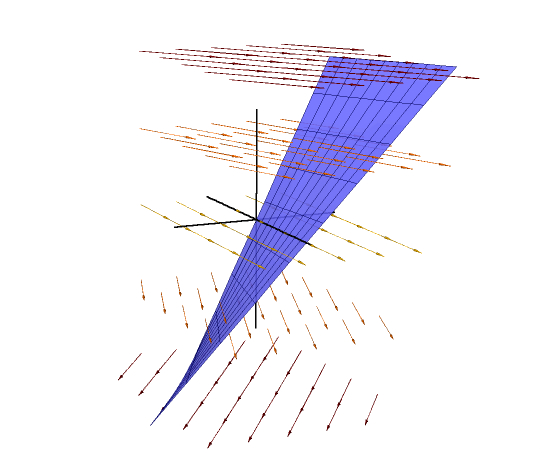
\includegraphics[width=200pt]{quasilinear-characteristics1.jpg} (b)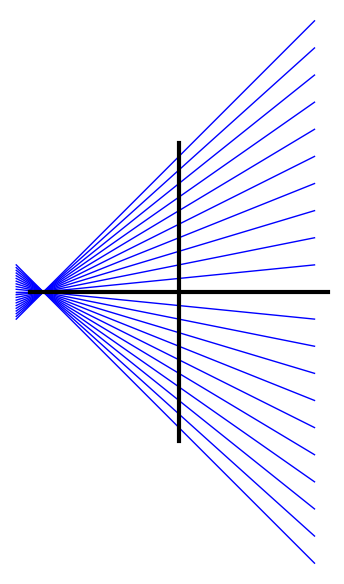
\includegraphics[width=150pt]{qcharacteristics1.png}
\end{center}
\caption{(a) The solution surface to $\frac{\partial\phi}{\partial x}+\phi\frac{\partial\phi}{\partial y}=0$ with the initial condition $\phi(0,y)=y$, plotted with the characteristic vector field. This surface is a union of straight lines which are characteristic curves. (b) The characteristic projections of this solution. You can see that they begin to cross at $(-1,0)$.}
\label{fig-quasilinear-characteristics-1}
\end{figure}

\begin{exm}\label{exm-burgers-2}
{\bf Solve the equation
\[\frac{\partial\phi}{\partial x}+\phi\frac{\partial\phi}{\partial y}\]
subject to the initial condition $\phi(0,s)=s^2$.}

We have the same characteristic curves
\[t\mapsto (t+c,at+b,a)\]
but a different initial condition $\phi(0,s)=s^2$. This gives
\[c=0,\ b=s,\ a=s^2\]
so the solution surface is parametrised by
\[(s,t)\mapsto (t,s^2t+s,s^2).\]
To express $z$ in terms of $x$ and $y$ we have to solve $y=s^2t+s$, $x=t$ for $s$. This gives
\[s=\frac{-1\pm \sqrt{1+4xy}}{2x}\]
or
\[z=\phi(x,y)=\left(\frac{-1\pm \sqrt{1+4xy}}{2x}\right)^2.\]
This fails to be well-defined when $x=0$ or when $1+4xy<0$.

If we draw the projections of the characteristic curves then we can see something strange happening in the vicinity of the curve $1+4xy=0$: the projections start to cross over and bunch up. The solution surface is folding over above this curve so it is not a graph there.
\end{exm}


\begin{figure}[htb]
\begin{center}
(a)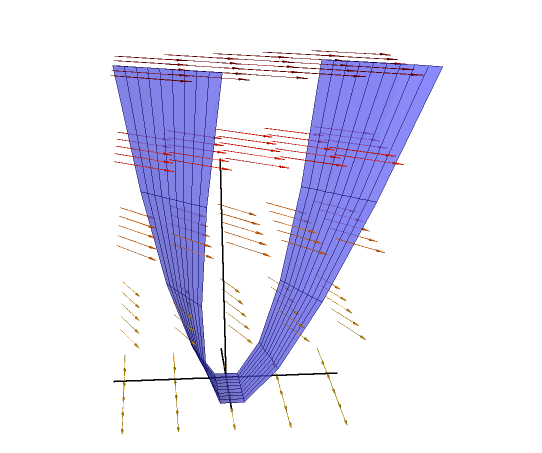
\includegraphics[width=200pt]{quasilinear-characteristics2.jpg} (b)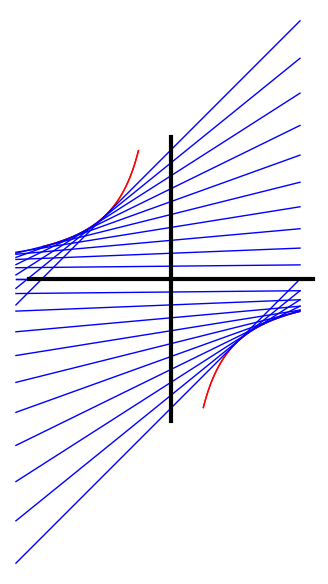
\includegraphics[width=150pt]{qcharacteristics2.png}
\end{center}
\caption{(a) The solution surface to $\frac{\partial\phi}{\partial x}+\phi\frac{\partial\phi}{\partial y}=0$ with initial condition $\phi(0,y)=y^2$, plotted with the characteristic vector field. You can see the graph starting to bend over and become double-valued. (b) The characteristic projections of this solution. You can see that they are all tangent to the red curve $1+4xy=0$ and that they are starting to cross one another near that curve.}
\label{fig-quasilinear-characteristics-2}
\end{figure}
\afterpage{\clearpage}

\section{Caustics}

\begin{dfn}
Let $(s,t)\mapsto(x(s,t),y(s,t),z(s,t))$ be a surface in $\RR^3$. The surface is said to have a vertical tangency at $(x,y,z)$ if some linear combination of the vectors
\[\left(\begin{array}{c}\partial x/\partial s\\\partial y/\partial s\\ \partial z/\partial s\end{array}\right)\mbox{ and }\left(\begin{array}{c}\partial x/\partial t\\\partial y/\partial t\\ \partial z/\partial t\end{array}\right)\]
gives
\[\left(\begin{array}{c}0\\0\\ 1\end{array}\right).\]
Take the set of points where the surface has a vertical tangency and project it to the $(x,y)$-plane. The image is called the {\em caustic} of the surface.
\end{dfn}

\begin{rmk}
The terminology ``caustic'' comes from optics: light travels along rays which are the projections of characteristic curves of a PDE called the eikonal equation. Along the caustic these rays bunch up and give rise to bright patches. The example we studied earlier was Burgers's equation and it arises in the study of waves: $\phi(x,y)$ is the velocity of fluid particles at the point $y$ at time $x$. In this context the caustics are called ``shocks'', where faster fluid particles overtake slower fluid particles.
\end{rmk}

Here is a method for finding the caustic.

\begin{dfn}
If $(s,t)\mapsto (x(s,t),y(s,t),z(s,t))$ is a parametrisation of a surface in $\RR^3$ then consider the projection $\pi(s,t)=(x(s,t),y(s,t))$. A point $(s,t)$ is called a critical point of $\pi$ if the {\em Jacobian determinant}
\[\det\left(\begin{array}{cc}\partial_sx & \partial_sy\\ \partial_tx & \partial_ty\end{array}\right)\]
vanishes. The image under $\pi$ of the set of critical points is called the set $C(\pi)$ of critical values.
\end{dfn}

\begin{lma}
The set $C(\pi)$ of critical values of the projection $\pi$ contains the caustic of the surface.
\end{lma}
\begin{proof}
If a point $(x_0,y_0)$ is in the caustic then there is an $(s,t)$ and coefficients $a,b$ such that
\[a\left(\begin{array}{c}\partial_sx\\\partial_sy\\\partial_sz\end{array}\right)+b\left(\begin{array}{c}\partial_tx\\\partial_ty\\\partial_tz\end{array}\right)=\left(\begin{array}{c}0\\0\\1\end{array}\right).\]
This implies that
\[a\left(\begin{array}{c}\partial_sx\\\partial_sy\end{array}\right)+b\left(\begin{array}{c}\partial_tx\\\partial_ty\end{array}\right)=0\]
so the vectors $\left(\begin{array}{c}\partial_sx\\\partial_sy\end{array}\right)$ and $\left(\begin{array}{c}\partial_tx\\\partial_ty\end{array}\right)$ are linearly dependent. This implies that the Jacobian determinant
\[\det\left(\begin{array}{cc}\partial_sx & \partial_sy\\ \partial_tx & \partial_ty\end{array}\right)\]
vanishes.
\end{proof}
\begin{rmk}
It is not always true that $C(\pi)$ equals the caustic: it is possible for the parametrisation of the surface itself to have a singularity so that the vectors
\[\left(\begin{array}{c}\partial_sx\\\partial_sy\\\partial_sz\end{array}\right)\mbox{ and }\left(\begin{array}{c}\partial_tx\\\partial_ty\\\partial_tz\end{array}\right)\]
are themselves linearly dependent.
\end{rmk}

\begin{exm}
Consider the solution surface $(s,t)\mapsto (t,st+s,s)$ we obtained as a solution to Example \ref{exm-burgers-1}. We have $\pi(s,t)=(t,st+s)$ so that the Jacobian determinant is
\[\det\left(\begin{array}{cc}0 & t+1\\ 1 & s\end{array}\right)=-(t+1).\]
This vanishes when $t=-1$ that is when $x=-1$, $y=0$. This is precisely the bad locus from earlier.
\end{exm}
\begin{exm}
Consider the solution surface $(s,t)\mapsto (t,s^2t+s,s^2)$ we obtained as a solution to Example \ref{exm-burgers-2}. We have $\pi(s,t)=(t,s^2t+s)$ so that the Jacobian determinant is
\[\det\left(\begin{array}{cc}0 & 2st+1\\ 1 & s^2\end{array}\right)=-(2st+1).\]
This vanishes when $2st+1=$, i.e. when $s=-1/2t$. This means $y=1/4t-1/2t=1/4x$, so $4xy+1=0$. This is part of the bad locus from earlier. The other part arose from the solution becoming infinite, not from the solution surface having a vertical tangency.
\end{exm}

\section{Another example}

\begin{exm}
{\bf Solve the PDE
\[-\sin\phi\frac{\partial\phi}{\partial x}+\cos\phi\frac{\partial\phi}{\partial y}=1\]
with initial condition
\[\phi(s,0)=0.\]}

The characteristic vector field is $(-\sin z,\cos z,1)$ and the characteristic curves are
\[z=t+c,\ x=\cos t+a,\ y=\sin t+b\]
These curves are helices spiralling upwards. The initial condition $\phi(s,0)=0$ along $t=0$ gives$c=0$, $s=1+a$, $0=b$ so the solution surface is parametrised by
\[(s,t)\mapsto (\cos t+s-1,\sin t,t).\]
We can express $z$ in terms of $x$ and $y$ easily:
\[z=\sin^{-1}y\]
but this is not a single-valued function so the solution surface is not a graph. If you draw the projections of the characteristic curves you get segments of circles centred on the $x$-axis with radius 1. These all become tangent to the curves $y=\pm 1$ which will turn out to the caustic.

The critical values of the projection are given by the vanishing of the determinant
\[\det\left(\begin{array}{cc}1 & 0\\-\sin t & \cos t\end{array}\right)=\cos t\]
so $t=(n+1/2)\pi$ for some $n\in\mathbf{Z}$. This gives $y=\pm 1$ as expected.
\end{exm}

\begin{figure}[htb]
\begin{center}
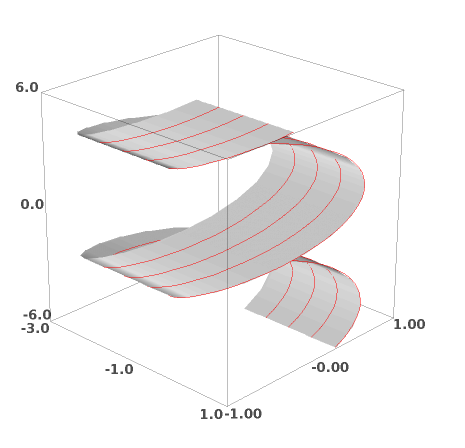
\includegraphics[width=300pt]{qcharacteristics4.png}
\end{center}
\caption{This is the solution surface parametrised by $(\cos t+s-1,\sin t,t)$ and some of the characteristic curves superimposed in red. The surface is folding over itself along the lines $y=\pm 1$.}
\label{fig-characteristics4}
\end{figure}

\begin{figure}[htb]
\begin{center}
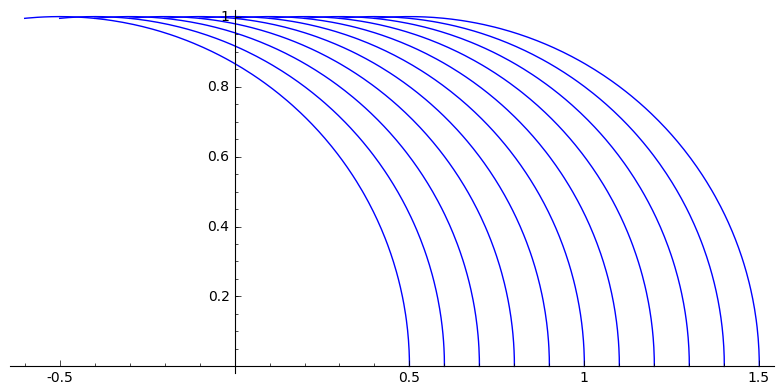
\includegraphics[width=300pt]{qcharacteristics3.png}
\end{center}
\caption{The characteristics of $-\sin\phi\frac{\partial\phi}{\partial x}+\cos\phi\frac{\partial\phi}{\partial y}=1$ are segments of circle. We see they start to overlap near $y=1$.}
\label{fig-characteristics3}
\end{figure}

\chapter[Method of characteristics, III]{* Method of characteristics, III: Fully nonlinear case (NONEXAMINABLE)}

The method works for the fully nonlinear case but the system of ODEs becomes yet more complicated.

\begin{leftbar}
Suppose that $G(x,y,u,p,q)$ is a function of five variables and that $\phi\colon\RR^2\to\RR$ is a function satisfying
\[G\left(x,y,\phi(x,y),\partial_x\phi(x,y),\partial_y\phi(x,y)\right)=0\]
for all $(x,y)\in\RR^2$. Now let $\gamma(t)=(x(t),y(t))$ be a curve and restrict $\phi$ to $\gamma$ to obtain a function $u(t)$ as usual. Let $G(t)$ denote
\[G(x(t),y(t),u(t),p(t),q(t))\]
where $p(t)=\partial_x\phi(x(t),y(t))$, $q(t)=\partial_y\phi(x(t),y(t))$. We have
\[\frac{dG}{dt}=\frac{\partial G}{\partial x}\dot{x}+\frac{\partial G}{\partial y}\dot{y}+\frac{\partial G}{\partial u}\dot{u}+\frac{\partial G}{\partial p}\dot{p}+\frac{\partial G}{\partial q}\dot{q}\]
and since $\dot{u}=\dot{x}\frac{\partial\phi}{\partial x}+\dot{y}\frac{\partial\phi}{\partial y}=\dot{x}p+\dot{y}q$ this becomes
\begin{align*}
\frac{dG}{dt}&=\dot{x}\left(\frac{\partial G}{\partial x}+\frac{\partial G}{\partial u}p\right)+\dot{y}\left(\frac{\partial G}{\partial y}+\frac{\partial G}{\partial u}q\right)+\\
&\ \ \ \ \ +\frac{\partial G}{\partial p}\dot{p}+\frac{\partial G}{\partial q}\dot{q}.
\end{align*}
This suggests a system of five coupled ODEs for the five quantities $(x(t),y(t),u(t),p(t),q(t))$:
\begin{align*}
\frac{dx}{dt}&=\frac{\partial G}{\partial p}&\dot{p}&=-\left(\frac{\partial G}{\partial x}+p\frac{\partial G}{\partial u}\right)\\
\frac{dy}{dt}&=\frac{\partial G}{\partial q}&\dot{q}&=-\left(\frac{\partial G}{\partial y}+q\frac{\partial G}{\partial u}\right)\\
&&\dot{u}&=\frac{\partial G}{\partial p}p+\frac{\partial G}{\partial q}q
\end{align*}
As usual, if we integrate this system of ODEs we will obtain a curve. Taking a one-parameter family of these integral curves gives a surface in $(x,y,u,p,q)$-space and when we project to $(x,y,u)$-space we obtain a surface which, wherever it is a graph, is the graph of a solution $u=\phi(x,y)$.
\end{leftbar}
\begin{figure}[htb]
\begin{center}
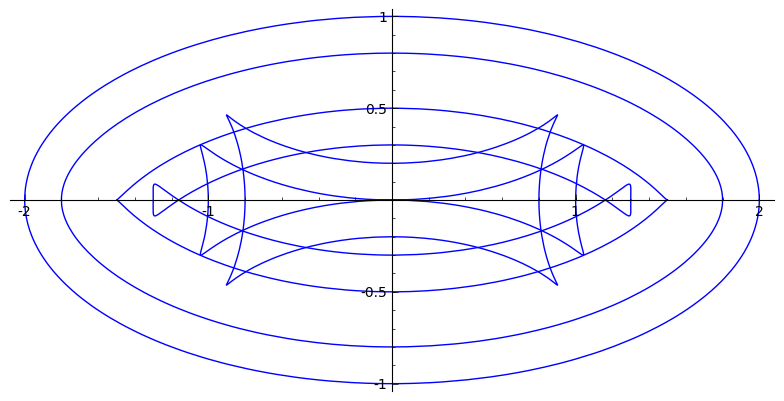
\includegraphics[width=300pt]{equidistants.png}
\end{center}
\caption{The equidistants of an ellipse form singularities as characteristics cross.}
\label{fig-equidistants}
\end{figure}
\begin{leftbar}
\begin{exm}
Let us consider the eikonal equation (in units where the speed of light is 1)
\[\left(\frac{\partial\phi}{\partial x}\right)^2+\left(\frac{\partial\phi}{\partial y}\right)^2=1\]
(so $G(x,y,u,p,q)=p^2+q^2$) which describes the time $\phi$ taken by light emitted normally by some curve $C\subset\RR^2$ to each a point $(x,y)\in\RR^2$. To see that this description is valid, let's consider the corresponding system of ODEs:
\begin{align*}
\frac{dx}{dt}&=2p&\dot{p}&=0\\
\frac{dy}{dt}&=2q&\dot{q}&=0\\
&&\dot{u}&=2(p^2+q^2)=2
\end{align*}
Starting from the curve $C$ and choose the initial condition $\phi|_C=0$. We see that this determines $p$ and $q$ along $C$, namely $(p,q)$ must be (plus or minus) the unit normal vector to the curve $C$ because $p^2+q^2=1$ (giving unit length) and because $(p,q)=\left(\tfrac{\partial\phi}{\partial x},\tfrac{\partial\phi}{\partial y}\right)$ and by our choice of initial condition the directional derivative of $\phi$ along $C$ vanishes, so $(p,q)$ is normal to $C$. Now along the integral curves of the ODE, $p$ and $q$ do not change and hence $x$ and $y$ follow the normal line (with speed 2) and the solution to $\dot{u}=2$ is just $u(t)=2t$. If one followed the normal with speed 1, we would get $u(t)=t$.

This is precisely the statement that the solution of the eikonal equation is the time taken by light to reach $(x,y)$ from $C$ in a normal direction. The characteristics are straight lines normal to $C$. Solutions of the eikonal equation can be very beautiful. Figure \ref{fig-equidistants} shows some of the singularities developed by level sets of $\phi$ corresponding to the initial condition $C=\left\{\frac{x^2}{4}+y^2=1\right\}$ (that is, the equidistants of an ellipse).
\end{exm}
\end{leftbar}


\chapter{D'Alembert's method}

In this final chapter we present one more situation in which a linear change of coordinates enables us to solve a PDE. This time we are interested in linear second-order hyperbolic equations with constant coefficients (and an arbitrary inhomogeneous term).

\section{The wave equation}

The wave equation
\[\frac{1}{c^2}\frac{\partial^2\phi}{\partial t^2}=\frac{\partial^2\phi}{\partial x^2}\]
is supposed to describe the motion of waves with speed $c$. The equation simplifies drastically if we change to so-called {\em light-cone coordinates}:
\[x_+=x+ct,\ x_-=x-ct.\]
The axis $x_-=0$ is a line where $x=ct$, in other words it is the trajectory of a particle moving with speed $c$ in the positive $x$-direction. Similarly the axis $x_+=0$ is the trajectory of a particle moving with speed $c$ in the negative $x$-direction. We have $x=\tfrac{1}{2}(x_++x_-)$ and $t=\tfrac{1}{2c}(x_+-x_-)$. Using the chain rule we have
\begin{align*}
\frac{\partial}{\partial x_{\pm}}&=\frac{\partial x}{\partial x_{\pm}}\frac{\partial}{\partial x}+\frac{\partial t}{\partial x_{\pm}}\frac{\partial}{\partial t}\\
&=\frac{1}{2}\left(\frac{\partial}{\partial x}\pm\frac{1}{c}\frac{\partial}{\partial t}\right)
\end{align*}
so
\[\frac{\partial^2}{\partial x^2}-\frac{1}{c^2}\frac{\partial^2}{\partial t^2}=4\frac{\partial^2}{\partial x_+\partial x_-}.\]
Therefore in these new coordinates the wave equation becomes
\[\frac{\partial^2\phi}{\partial x_+\partial x_-}=0\]
Integrating this directly we see that $\phi(x_-,x_+)=C_-(x_-)+C_+(x_+)$ for arbitrary functions $C_{\pm}$. In other words, {\em any solution to the wave equation can be written as}
\[\phi(x,t)=C_-(x-ct)+C_+(x+ct).\]
We think of the first term as a {\em right-moving wave} and the second as a {\em left-moving wave}. Imagine for example that $C_-=\cos$ and observe that $\cos$ has a local maximum (`crest') at zero. Therefore $C_-(x-ct)$ has a crest at $x-ct=0$, so the crest of this wave moves along the trajectory $x=ct$ of a right-moving particle with speed $c$.

\begin{exm}
{\bf Solve the wave equation for $\phi(x,t)$ with initial conditions}
\[\phi(x,0)=e^{-x^2},\qquad\frac{\partial\phi}{\partial t}(x,0)=0.\]
We know that the solution has the form
\[\phi(x,t)=C_-(x-ct)+C_+(x+ct).\]
The initial conditions become
\[\phi(x,0)=C_-(x)+C_+(x)=e^{-x^2},\qquad\frac{\partial\phi}{\partial t}(x,0)=-cC'_-(x)+cC'_+(x)=0.\]
This gives us two simultaneous equations for $C_{\pm}$. Integrating the second equation implies $C_+(x)=C_-(x)+k$ for some constant $k$. The first then gives
\[C_-(x)+C_+(x)=2C_-(x)+k=e^{-x^2}\]
so $C_-(x)=\frac{1}{2}\left(e^{-x^2}-k\right)$ and $C_+(x)=\frac{1}{2}\left(e^{-x^2}+k\right)$. The solution is therefore
\[\frac{1}{2}\left(e^{-(x-ct)^2}+e^{-(x+ct)^2}\right),\]
in other words, the initial (Gaussian) wave splits into two components with half the amplitude, one moving right, one moving left. Note that the constant $k$ cancelled out. This will always be the case, so we will never bother to include it in our calculations.
\end{exm}

\begin{rmk}[Comparison of Fourier and d'Alembert]
Fourier's (separated) solutions to the wave equation have the form
\[\sin(px)\sin(pct).\]
D'Alembert tells us that we can write this as a sum of a right-moving and a left-moving wave. We can do this explicitly using the trigonometric identities, and we get
\[\sin(px)\sin(pct)=\frac{1}{2}\left(\cos p(x-ct)-\cos p(x+ct)\right).\]
\end{rmk}

\section{Hyperbolic equations}

The wave equation belongs to the class of hyperbolic second-order linear equations. We will consider the most general of these in two variables $x,y$:
\[A\frac{\partial^2\phi}{\partial x^2}+B\frac{\partial^2\phi}{\partial x\partial y}+C\frac{\partial^2\phi}{\partial y^2}=D(x,y)\]
where $A,B,C$ are constants (suppose for simplicity that $A\neq 0$) and $D$ is a function of $x$ and $y$. We will find coordinates $(s,t)$ so that the equation becomes
\[A\frac{\partial^2\phi}{\partial s\partial t}=D\]
in other words, we need to find $(s,t)$ so that
\[A\frac{\partial^2}{\partial s\partial t}=A\frac{\partial^2\phi}{\partial x^2}+B\frac{\partial^2\phi}{\partial x\partial y}+C\frac{\partial^2\phi}{\partial y^2}.\]
The following lemma is good practice in using the chain rule:
\begin{lma}
If we have
\[x=s+t,\qquad y=-\beta s-\alpha t\]
then
\[\frac{\partial^2}{\partial s\partial t}=\frac{\partial^2}{\partial x^2}-(\alpha+\beta)\frac{\partial^2}{\partial x\partial y}+\alpha\beta\frac{\partial^2}{\partial y^2}.\]
\end{lma}
\begin{proof}
We have
\[\frac{\partial}{\partial s}=\frac{\partial x}{\partial s}\frac{\partial}{\partial x}+\frac{\partial y}{\partial s}\frac{\partial}{\partial y}=\frac{\partial}{\partial x}-\beta\frac{\partial}{\partial y}\]
and
\[\frac{\partial}{\partial t}=\frac{\partial x}{\partial t}\frac{\partial}{\partial x}+\frac{\partial y}{\partial t}\frac{\partial}{\partial y}=\frac{\partial}{\partial x}-\alpha\frac{\partial}{\partial y}\]
so
\begin{align*}
\frac{\partial^2}{\partial s\partial t}&=\left(\frac{\partial}{\partial x}-\beta\frac{\partial}{\partial y}\right)\left(\frac{\partial}{\partial x}-\alpha\frac{\partial}{\partial y}\right)\\
&=\frac{\partial^2}{\partial x^2}-(\alpha+\beta)\frac{\partial^2}{\partial x\partial y}+\alpha\beta\frac{\partial^2}{\partial y^2}
\end{align*}
\end{proof}

We will choose $\alpha$ and $\beta$ so that
\[A\frac{\partial^2}{\partial s\partial t}=A\frac{\partial^2}{\partial x^2}+B\frac{\partial^2}{\partial x\partial y}+C\frac{\partial^2}{\partial y^2}\]
that is
\[B/A=-(\alpha+\beta),\qquad C/A=\alpha\beta.\]
\begin{lma}
If $\alpha$ and $\beta$ are the roots of the quadratic equation
\[AT^2+BT+C=0\]
then $B/A=-(\alpha+\beta)$ and $C/A=\alpha\beta$.
\end{lma}
\begin{proof}
The quadratic equation with roots $\alpha$ and $\beta$ and top coefficient $AT^2$ is $A(T-\alpha)(T-\beta)$. Multiplying this out gives $A(T^2-(\alpha+\beta)T+\alpha\beta)$ so $B/A=-(\alpha+\beta)$ and $C/A=\alpha\beta$.
\end{proof}
\begin{dfn}
A PDE
\[A\ppd{\phi}{x}+B\ppdd{\phi}{x}{y}+C\ppd{\phi}{y}=D\]
is said to be hyperbolic, parabolic or elliptic if the quantity $B^2-4AC$ is, respectively, positive, zero or negative.
\end{dfn}
\begin{rmk}
If the PDE is hyperbolic then the roots of $AT^2+BT+C$ are $\tfrac{1}{2A}\left(-B\pm\sqrt{B^2-4AC}\right)$ which are distinct and real. This guarantees that $x=s+t$, $y=-\beta s-\alpha t$ is a well-defined change of coordinates.
\end{rmk}
In conclusion:
\begin{prp}
If
\[A\ppd{\phi}{x}+B\ppdd{\phi}{x}{y}+C\ppd{\phi}{y}=D\]
is a hyperbolic PDE and $\alpha,\beta$ are the roots of $AT^2+BT+C=0$ then under the change of coordinates
\[x=s+t,\qquad y=-\beta s-\alpha t\]
the PDE simplifies to
\[A\ppdd{\phi}{s}{t}=D.\]
\end{prp}

\begin{exm}
{\bf Solve}
\[\frac{\partial^2\phi}{\partial x^2}+5\frac{\partial^2\phi}{\partial x\partial y}+4\frac{\partial^2\phi}{\partial y^2}=xy\]
The quadratic equation we need to solve is $T^2+5T+4=0$ which has roots $(-5\pm\sqrt{25-16})/2$ that is $\alpha=-4$, $\beta=-1$. Under the change of coordinates $x=s+t$, $y=s+4t$ (equivalently $s=\tfrac{1}{3}(4x-y)$, $t=\tfrac{1}{3}(y-x)$) the PDE becomes
\[\frac{\partial^2\phi}{\partial s\partial t}=xy=s^2+5st+4t^2\]
so integrating up directly we get
\[\phi(s,t)=\frac{1}{3}s^3t+\frac{5}{4}s^2t^2+\frac{4}{3}st^3+C_1(s)+C_2(t)\]
where $C_1$ and $C_2$ are arbitrary functions. Changing coordinates back to $x,y$ we have
\begin{align*}
\phi(x,y)&=\frac{1}{81}\left(\frac{1}{3}(4x-y)^3(y-x)+\frac{5}{4}(4x-y)^2(y-x)^2+\frac{4}{3}(4x-y)(y-x)^3\right)\\
&\ \ \ \ \ +C_1((4x-y)/3)+C_2((y-x)/3).
\end{align*}
\end{exm}

\begin{exm}
{\bf Solve}
\[\frac{\partial^2\phi}{\partial x^2}+5\frac{\partial^2\phi}{\partial x\partial y}+4\frac{\partial^2\phi}{\partial y^2}=0\]
{\bf subject to the conditions}
\[\phi(x,0)=x,\qquad\frac{\partial\phi}{\partial y}(x,0)=x^2\]
We have already found the relevant coordinates for this equation in the previous example $s=\tfrac{1}{3}(4x-y)$, $t=\tfrac{1}{3}(y-x)$. With these coordinates the equation becomes
\[\frac{\partial^2\phi}{\partial s\partial t}=0\]
so $\phi(s,t)=C_1(s)+C_2(t)$ or
\[\phi(x,y)=C_1\left(\frac{1}{3}(4x-y)\right)+C_2\left(\frac{1}{3}(y-x)\right).\]
The condition $\phi(x,0)=x$ gives
\[C_1(4x/3)+C_2(-x/3)=x\]
and the condition $\partial\phi/\partial y(x,0)=x^2$ gives
\[-\frac{1}{3}C'_1(4x/3)+\frac{1}{3}C'_2(-x/3)=x^2.\]
Integrating this second equation gives\footnote{Again we are ignoring a constant here because if we included it, it would cancel out later.}
\[-\frac{3}{4}C_1(4x/3)-3C_2(-x/3)=x^3\]
Now we have two simultaneous equations for $C_1$ and $C_2$. These give
\[(3-4/3)C_1(4x/3)=3x+x^3,\qquad (3/4-3)C_2(-x/3)=3x/4+x^3\]
or
\[C_1(4x/3)=4(x^3+3x)/9,\qquad C_2(-x/3)=-4(x^3+3x/4)/9.\]
Substituting $u=4x/3$ we get
\[C_1(u)=u+\frac{3u^3}{16}\]
and substituting $u=-x/3$ we get
\[C_2(u)=u+12u^3.\]
Therefore the final solution, $\phi(s,t)=C_1(s)+C_2(t)$, is
\[\phi(x,y)=\left(\frac{1}{3}(4x-y)+\frac{3}{16}\left(\frac{1}{3}(4x-y)\right)^3\right)+\left(\frac{1}{3}(y-x)+12\left(\frac{1}{3}(y-x)\right)^3\right).\]
\end{exm}

%%% Local Variables: 
%%% mode: latex
%%% TeX-master: "notes"
%%% End: 

\end{document}



